\batchmode

\documentclass[a4j,10pt]{jsarticle}
\RequirePackage{ifthen}


\usepackage{datetime2}
\usepackage[dvipdfmx]{graphicx,color}
\usepackage[dvipdfmx,setpagesize=true,bookmarksnumbered=true,colorlinks=true]{hyperref}
\usepackage[utf8]{inputenc}
\usepackage{okumacro} 
\usepackage{dcolumn}
\usepackage{booktabs}
\usepackage{setspace}
\usepackage{relsize}
\usepackage{comment}
\usepackage{latexsym}
\usepackage{amsmath,amsthm,amssymb}
\usepackage{itembkbx}
\usepackage{itembbox}
\usepackage{ascmac}
\usepackage{pxjahyper}     
\usepackage{longtable}
\DeclareUnicodeCharacter{22EE}{\vdots} % vertical dots in the middle of the Julia output
\usepackage{minted}
\RequirePackage{fancyvrb}
\DefineVerbatimEnvironment{verbatim}{Verbatim}{fontsize=\scriptsize ,formatcom={\color{red}},frame=single}
\usetheme{default}
\author{菅野 剛}
\date{\DTMnow}
\title{日本大学文理学部社会学科 Blackboard FAQ 非公式}
\hypersetup{
 pdfauthor={菅野 剛},
 pdftitle={日本大学文理学部社会学科 Blackboard FAQ 非公式},
 pdfkeywords={},
 pdfsubject={},
 pdfcreator={Emacs 27.1 (Org mode 9.4.4)}, 
 pdflang={Ja}}


\usepackage[]{inputenc}



\makeatletter

\makeatletter
\count@=\the\catcode`\_ \catcode`\_=8 
\newenvironment{tex2html_wrap}{}{}%
\catcode`\<=12\catcode`\_=\count@
\newcommand{\providedcommand}[1]{\expandafter\providecommand\csname #1\endcsname}%
\newcommand{\renewedcommand}[1]{\expandafter\providecommand\csname #1\endcsname{}%
  \expandafter\renewcommand\csname #1\endcsname}%
\newcommand{\newedenvironment}[1]{\newenvironment{#1}{}{}\renewenvironment{#1}}%
\let\newedcommand\renewedcommand
\let\renewedenvironment\newedenvironment
\makeatother
\let\mathon=$
\let\mathoff=$
\ifx\AtBeginDocument\undefined \newcommand{\AtBeginDocument}[1]{}\fi
\newbox\sizebox
\setlength{\hoffset}{0pt}\setlength{\voffset}{0pt}
\addtolength{\textheight}{\footskip}\setlength{\footskip}{0pt}
\addtolength{\textheight}{\topmargin}\setlength{\topmargin}{0pt}
\addtolength{\textheight}{\headheight}\setlength{\headheight}{0pt}
\addtolength{\textheight}{\headsep}\setlength{\headsep}{0pt}
\setlength{\textwidth}{349pt}
\newwrite\lthtmlwrite
\makeatletter
\let\realnormalsize=\normalsize
\global\topskip=2sp
\def\preveqno{}\let\real@float=\@float \let\realend@float=\end@float
\def\@float{\let\@savefreelist\@freelist\real@float}
\def\liih@math{\ifmmode$\else\bad@math\fi}
\def\end@float{\realend@float\global\let\@freelist\@savefreelist}
\let\real@dbflt=\@dbflt \let\end@dblfloat=\end@float
\let\@largefloatcheck=\relax
\let\if@boxedmulticols=\iftrue
\def\@dbflt{\let\@savefreelist\@freelist\real@dbflt}
\def\adjustnormalsize{\def\normalsize{\mathsurround=0pt \realnormalsize
 \parindent=0pt\abovedisplayskip=0pt\belowdisplayskip=0pt}%
 \def\phantompar{\csname par\endcsname}\normalsize}%
\def\lthtmltypeout#1{{\let\protect\string \immediate\write\lthtmlwrite{#1}}}%
\usepackage[tightpage,active]{preview}
\newbox\lthtmlPageBox
\newdimen\lthtmlCropMarkHeight
\newdimen\lthtmlCropMarkDepth
\long\def\lthtmlTightVBoxA#1{\def\lthtmllabel{#1}
    \setbox\lthtmlPageBox\vbox\bgroup\hbox\bgroup\catcode`\_=8 }%
\long\def\lthtmlTightVBoxZ{\egroup\egroup
    \lthtmlCropMarkHeight=\ht\lthtmlPageBox \advance \lthtmlCropMarkHeight 6pt
    \lthtmlCropMarkDepth=\dp\lthtmlPageBox
    \lthtmltypeout{^^J:\lthtmllabel:lthtmlCropMarkHeight:=\the\lthtmlCropMarkHeight}%
    \lthtmltypeout{^^J:\lthtmllabel:lthtmlCropMarkDepth:=\the\lthtmlCropMarkDepth:1ex:=\the \dimexpr 1ex}%
    \begin{preview}\copy\lthtmlPageBox\end{preview}}%
\long\def\lthtmlTightFBoxA#1{\def\lthtmllabel{#1}%
    \adjustnormalsize\setbox\lthtmlPageBox=\vbox\bgroup %
    \let\ifinner=\iffalse \let\)\liih@math %
    \bgroup\catcode`\_=8 }%
\long\def\lthtmlTightFBoxZ{\egroup
    \@next\next\@currlist{}{\def\next{\voidb@x}}%
    \expandafter\box\next\egroup %
    \lthtmlCropMarkHeight=\ht\lthtmlPageBox \advance \lthtmlCropMarkHeight 6pt
    \lthtmlCropMarkDepth=\dp\lthtmlPageBox
    \lthtmltypeout{^^J:\lthtmllabel:lthtmlCropMarkHeight:=\the\lthtmlCropMarkHeight}%
    \lthtmltypeout{^^J:\lthtmllabel:lthtmlCropMarkDepth:=\the\lthtmlCropMarkDepth:1ex:=\the \dimexpr 1ex}%
    \begin{preview}\copy\lthtmlPageBox\end{preview}}%
    \long\def\lthtmlinlinemathA#1#2\lthtmlindisplaymathZ{\lthtmlTightVBoxA{#1}{#2}\lthtmlTightVBoxZ}
    \def\lthtmlinlineA#1#2\lthtmlinlineZ{\lthtmlTightVBoxA{#1}{#2}\lthtmlTightVBoxZ}
    \long\def\lthtmldisplayA#1#2\lthtmldisplayZ{\lthtmlTightVBoxA{#1}{#2}\lthtmlTightVBoxZ}
    \long\def\lthtmldisplayB#1#2\lthtmldisplayZ{\\edef\preveqno{(\theequation)}%
        \lthtmlTightVBoxA{#1}{\let\@eqnnum\relax#2}\lthtmlTightVBoxZ}
    \long\def\lthtmlfigureA#1{\let\@savefreelist\@freelist
        \lthtmlTightFBoxA{#1}}
    \long\def\lthtmlfigureZ{
        \lthtmlTightFBoxZ\global\let\@freelist\@savefreelist}
    \long\def\lthtmlpictureA#1{\let\@savefreelist\@freelist
        \lthtmlTightVBoxA{#1}}
    \long\def\lthtmlpictureZ{
        \lthtmlTightVBoxZ\global\let\@freelist\@savefreelist}
\def\lthtmlcheckvsize{\ifdim\ht\sizebox<\vsize 
  \ifdim\wd\sizebox<\hsize\expandafter\hfill\fi \expandafter\vfill
  \else\expandafter\vss\fi}%
\providecommand{\selectlanguage}[1]{}%
\makeatletter \tracingstats = 1 
\providecommand{\Beta}{\textrm{B}}
\providecommand{\Zeta}{\textrm{Z}}
\providecommand{\Epsilon}{\textrm{E}}
\providecommand{\Iota}{\textrm{J}}
\providecommand{\Tau}{\textrm{T}}
\providecommand{\Alpha}{\textrm{A}}
\providecommand{\omicron}{\textrm{o}}
\providecommand{\Nu}{\textrm{N}}
\providecommand{\Omicron}{\textrm{O}}
\providecommand{\Rho}{\textrm{R}}
\providecommand{\Eta}{\textrm{H}}
\providecommand{\Mu}{\textrm{M}}
\providecommand{\Chi}{\textrm{X}}
\providecommand{\Kappa}{\textrm{K}}


\begin{document}
\pagestyle{empty}\thispagestyle{empty}\lthtmltypeout{}%
\lthtmltypeout{latex2htmlLength hsize=\the\hsize}\lthtmltypeout{}%
\lthtmltypeout{latex2htmlLength vsize=\the\vsize}\lthtmltypeout{}%
\lthtmltypeout{latex2htmlLength hoffset=\the\hoffset}\lthtmltypeout{}%
\lthtmltypeout{latex2htmlLength voffset=\the\voffset}\lthtmltypeout{}%
\lthtmltypeout{latex2htmlLength topmargin=\the\topmargin}\lthtmltypeout{}%
\lthtmltypeout{latex2htmlLength topskip=\the\topskip}\lthtmltypeout{}%
\lthtmltypeout{latex2htmlLength headheight=\the\headheight}\lthtmltypeout{}%
\lthtmltypeout{latex2htmlLength headsep=\the\headsep}\lthtmltypeout{}%
\lthtmltypeout{latex2htmlLength parskip=\the\parskip}\lthtmltypeout{}%
\lthtmltypeout{latex2htmlLength oddsidemargin=\the\oddsidemargin}\lthtmltypeout{}%
\makeatletter
\if@twoside\lthtmltypeout{latex2htmlLength evensidemargin=\the\evensidemargin}%
\else\lthtmltypeout{latex2htmlLength evensidemargin=\the\oddsidemargin}\fi%
\lthtmltypeout{}%
\makeatother
\setcounter{page}{1}
\onecolumn

% !!! IMAGES START HERE !!!

\setcounter{tocdepth}{2}
{\newpage\clearpage
\lthtmlfigureA{frame42}%
\begin{frame}
% latex2html id marker 42
[label={sec:orgc30a9e5},fragile]{概要}
\begin{block}{概要}
\begin{itemize}
\item リンクはトップページ \url{https://sugano-lab.github.io/blackboard-faq/} にして下さい。更新頻度は低いです。
\begin{itemize}
\item 1ページで全てを閲覧: \url{https://sugano-lab.github.io/blackboard-faq/blackboard-faq-all.html}
\item PDFで閲覧: \url{https://sugano-lab.github.io/blackboard-faq/blackboard-faq.pdf}
\end{itemize}
\item 遠隔授業実施に伴う、 Blackboard 等でのお問い合わせと回答に関するメモ (未整理・重複あり)
\begin{itemize}
\item \href{https://www.chs.nihon-u.ac.jp/}{文理学部HP} / \href{https://comits2.educ.chs.nihon-u.ac.jp/uniprove\_pt/UnLoginAction}{COMITS2} / 学内文書による通達 / \href{https://nuchs.blackboard.com/webapps/blackboard/execute/launcher?type=Course\&id=\_2302\_1\&url=}{Blackboard 20204702 : 遠隔授業サポート(社会学科)} / \href{http://dep.chs.nihon-u.ac.jp/sociology/index.htm}{社会学科HP} / \href{http://dep.chs.nihon-u.ac.jp/sociology/form.html}{社会学科メールお問い合わせフォーム} / \href{https://sites.google.com/a/nihon-u.ac.jp/nusocio/home}{nusocio 日本大学文理学部社会学科【新年度情報】} / 電話による対応 等にまたがる情報
\end{itemize}
\par
\item 内容について正確さの保証はありません
\begin{enumerate}
\item 作成者は、 Blackboard、 Microsoft Windows 、 Word をあまり使いません
\item 匿名のお問い合せが多く、フィードバックも得られないため、解決したのかどうか不明です
\end{enumerate}
\end{itemize}
\end{block}
\par
\begin{block}{注意}
\begin{figure}[htbp]
\centering
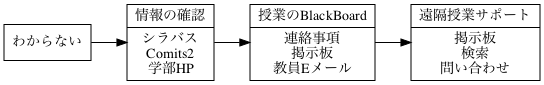
\includegraphics[height=2cm]{figures/blackboard-faq-dot-01.png}
\caption{
遠隔授業での質問}
\end{figure}
\par
\begin{itemize}
\item 遠隔授業についての質問は、基本的には、授業担当の教員が対応
\begin{enumerate}
\item \href{https://syllabus.chs.nihon-u.ac.jp/}{シラバス} 、 \href{https://comits2.educ.chs.nihon-u.ac.jp/uniprove\_pt/UnLoginAction}{Comits2} 、 \href{https://www.chs.nihon-u.ac.jp/}{学部HP} を確認
\begin{itemize}
\item 授業の \alert{シラバスを確認} を必ずしましょう
\end{itemize}
\par
\item 履修している授業の \href{https://nuchs.blackboard.com/}{Blackboard} のコースを確認
\begin{itemize}
\item \alert{連絡事項} 、 \alert{掲示板} を確認
\item 授業の Blackboard のEメールで授業担当教員へ問い合わせ
\item Google Classroom のコメント、限定公開コメント、Googleフォーム等で授業担当教員へ問い合わせ
\end{itemize}
\par
\item 遠隔授業サポート(社会学科)
\begin{itemize}
\item Blackboard \href{https://nuchs.blackboard.com/webapps/blackboard/execute/modulepage/view?course\_id=\_2302\_1\&cmp\_tab\_id=\_4690\_1\&mode=view}{遠隔授業サポート(社会学科)} の \alert{掲示板} で \alert{検索} し、過去の回答を参考にして下さい
\item 2020年度前期の問いあわせと対応については、この Webページにもまとめました (2020年度後期は未反映)
\item \alert{ページ内検索} をすれば、過去の情報を再利用・活用できます
\item 解決しない場合、 \href{https://nuchs.blackboard.com/webapps/blackboard/execute/modulepage/view?course\_id=\_2302\_1\&cmp\_tab\_id=\_4690\_1\&mode=view}{遠隔授業サポート(社会学科)} の \alert{掲示板} へ問い合わせ
\begin{itemize}
\item \href{https://nuchs.blackboard.com/webapps/blackboard/execute/modulepage/view?course\_id=\_2302\_1\&cmp\_tab\_id=\_4690\_1\&mode=view}{遠隔授業サポート(社会学科)} へのEメールによるお問い合わせは、御遠慮ください (情報共有・作業連携が進まない、責任の所在が不明)
\end{itemize}
\item \alert{掲示板} には、記名でも匿名でも、書き込みができます
\item 問い合わせをする場合、 \alert{状況判断と解決に必要な具体的情報を含める} こと
\item 知っていること、解決できることは、 \alert{学生同士で回答} し、助けあって下さい
\item 解決した / 解決しなかったなどのフィードバックも、重要な貢献です
\end{itemize}
\end{enumerate}
\end{itemize}
\par
\begin{itemize}
\item 文理学部内の他学科でも、同様の問い合わせと対応が発生していると思われるので、他学科での \alert{問い合わせや回答の情報を共有} する枠組みが望ましい
\par
\item 社会学科と別の総合教育科目への問い合わせや、語学科目への問い合わせ、管轄外の総合教育科目についての他学科学生からの電話問い合わせについては、改善・効率化の余地がある
\end{itemize}
\end{block}
\par
\begin{block}{キーワード指定でページ内検索}
\begin{itemize}
\item Webページ内全て確認するのは大変。キーワード指定で \alert{ページ内検索} 。
\begin{itemize}
\item Google Chrome ブラウザ: \href{https://support.google.com/chromebook/answer/95440?co=GENIE.Platform\%3DDesktop\&hl=ja}{Chrome でウェブを検索する - パソコン - Chromebook ヘルプ}
\item iPhone Safari :\href{https://support.apple.com/ja-jp/guide/iphone/iph6297b394b/ios}{iPhoneでSafariを使用してWebサイトを検索する - Apple サポート} の最後辺りの「ページ内を検索する」(ページで特定の語句を検索できます。) を参照
\item アンドロイド Chrome アプリ: \href{https://support.google.com/chrome/answer/95440?co=GENIE.Platform\%3DAndroid\&hl=ja}{Chrome でウェブを検索する - Android - Google Chrome ヘルプ} の「ウェブページ内を検索する」を参照
\item Windows : Webブラウザで【Ctrl】を押しながら【F】キーを押し、キーワードを入力
\item Mac : Webブラウザで【command】キーを押しながら【F】キーを押し、キーワードを入力
\end{itemize}
\end{itemize}
\end{block}
\end{frame}%
\lthtmlfigureZ
\lthtmlcheckvsize\clearpage}

{\newpage\clearpage
\lthtmlfigureA{frame132}%
\begin{frame}[label={sec:orgb5859c3},fragile]{個別の授業}
個別の授業についての対応情報・記録は、この Webページでの掲載は控えさせて頂きます
\par
\begin{enumerate}
\item 個別授業への問い合わせ → 授業担当の教員へ、 Blackboard の掲示板や Eメールで問い合わせて下さい。
\begin{itemize}
\item ただし、質問の内容によっては、返事を必ずしも得られるとは限りません。
\end{itemize}
\par
\item 総合教育科目への問い合わせ → 担当の幹事学科へ問い合わせ
\begin{enumerate}
\item \href{https://syllabus.chs.nihon-u.ac.jp/op/list1\_1.html}{総合教育科目 総合I群 シラバス}
\item \href{https://syllabus.chs.nihon-u.ac.jp/op/list1\_2.html}{総合教育科目 総合II群 シラバス}
\item \href{https://syllabus.chs.nihon-u.ac.jp/op/list1\_3.html}{総合教育科目 総合III群 シラバス}
\end{enumerate}
\par
\item 語学科目への問い合わせ → 日本大学文理学部外国語教育センターへ問い合わせ
\begin{itemize}
\item \href{https://www.chs.nihon-u.ac.jp/contact/flec\_form/}{日本大学文理学部 | 日本大学文理学部外国語教育センター(お問い合わせ)}
\end{itemize}
\end{enumerate}
\end{frame}%
\lthtmlfigureZ
\lthtmlcheckvsize\clearpage}

{\newpage\clearpage
\lthtmlfigureA{frame152}%
\begin{frame}[label={sec:org810c794},fragile]{新型コロナ感染症}
\begin{block}{新型コロナ感染症と学業}
\begin{itemize}
\item 新型コロナ感染症と診断されました。テスト、レポート課題、卒業論文をどうすればいいですか。
\item 無理をして外出や通学をしないようにして下さい。
\item 早めにご報告、ご相談し、対応をして下さい。
\end{itemize}
\par
\begin{block}{新型コロナウイルス感染症に係る本学部の対応について(2020/3/5時点)}
「感染者」及び「濃厚接触者」の取扱いについて
\par
感染が疑われ検査を行った場合は、検査結果を必ず文理学部学生課に報告してください。
\begin{itemize}
\item 報告内容
\begin{enumerate}
\item 医療機関受診日
\item 検査結果確定日
\item 病状の詳細等
\end{enumerate}
\item 新型コロナウイルス感染症に罹患した場合は、学校保健安全法施行規則第19条により、治癒するまで「出席停止」となります。
\item 検査の結果が陰性の場合は通常の病欠と同様の処理とします。
\end{itemize}
\end{block}
\par
\begin{block}{日本大学文理学部の対応 (2020/4/8時点)}
\begin{itemize}
\item \href{https://www.chs.nihon-u.ac.jp/student/2020-04-08/15016/}{日本大学文理学部 | 【学生の皆様へ】新型コロナウイルス感染症に係る本学部の対応について《4月8日(水)現在》}
\end{itemize}
\end{block}
\end{block}
\end{frame}%
\lthtmlfigureZ
\lthtmlcheckvsize\clearpage}

{\newpage\clearpage
\lthtmlfigureA{frame175}%
\begin{frame}[label={sec:org92b203c},fragile]{Blackboard へのログイン}
\begin{block}{ログイン}
\begin{block}{どの Webページからログインをするのでしょうか?}
\begin{itemize}
\item 文理学部の Blackboard は、 Amazon AWS を利用するクラウド環境へ移行しました。
\begin{itemize}
\item \url{https://nuchs.blackboard.com/}
\end{itemize}
\par
\item 文理学部の以前の Blackboard も、自分の Eメール確認用途などで利用します。
\begin{itemize}
\item \url{https://minerva3.educ.chs.nihon-u.ac.jp/}
\end{itemize}
\end{itemize}
\end{block}
\par
\begin{block}{ログインのアカウントとパスワードがわかりせん}
\begin{itemize}
\item ログインするには、文理学部の Microsoft Office365 Outlook メールアドレスが必要です。
\item Microsoft Office365 Outlook メールは、 \url{https://mail.office365.com/} からログインして利用する、文理学部のメールで、xxx[at]stu.chs.nihon-u.ac.jpです。
\item 日本大学本部の NU-AppsG メールxxx[at]g.nihon-u.ac.jpでは、 Blackboard にログインできませんので、ご注意下さい。
\end{itemize}
\end{block}
\par
\begin{block}{ログインすると、エラー表示}
\begin{itemize}
\item Windows の Internet Explorer など古い Webブラウザを利用すると、ログインでエラーになります。
\item 推奨ブラウザである Google Chrome の最新バージョンをインストールし、利用してみて下さい。
\begin{itemize}
\item \url{https://www.google.com/intl/ja\_jp/chrome/}
\end{itemize}
\end{itemize}
\end{block}
\end{block}
\end{frame}%
\lthtmlfigureZ
\lthtmlcheckvsize\clearpage}

{\newpage\clearpage
\lthtmlfigureA{frame207}%
\begin{frame}[label={sec:orgda0915a},fragile]{Blackboard のコース}
\begin{block}{コースの検索}
\begin{block}{履修する授業のコースを検索しても、見つからない}
\begin{itemize}
\item 稀に、 Blackboard でのコース名が、シラバス上の授業科目名の表記と、若干異なることがあります。
\item シラバスで授業科目名、担当教員名を調べ、それらの一部をキーワードとして、検索を行ってみてください。
\item 検索は、ちょっとコツがいる感じです。
\item いろいろ試してみて見てください。
\end{itemize}
\end{block}
\end{block}
\par
\begin{block}{コースの登録}
\begin{block}{履修する授業のコースを見つけたが、登録できない}
\begin{itemize}
\item 教員側が、何らかの事情で、まだ登録可能にしていないことが可能性として考えられます。
\item 登録が出来るはずの時期なのに、登録ができない場合は、学科事務室経由で、授業担当教員に連絡をとることになります。
\end{itemize}
\end{block}
\par
\begin{block}{履修する授業のコースに登録したのですが、教材がなく、授業に参加できない}
\begin{itemize}
\item 履修する授業の、前年度 (2019年度等) のコースなどに登録をしていないか、確認をして下さい。
\item ややこしいのですが、 Blackboard では、同じ名前の過去の授業も見えてしまい、間違って登録してしまうことがあります。
\item 同じ名前で、 2020年度のコースであることを確認して、登録をして下さい。
\end{itemize}
\end{block}
\par
\begin{block}{履修する授業のコースから、いつの間にか登録解除されていた}
\begin{itemize}
\item 授業によっては、受講者を何らかの基準で選別するということがあるかもしれませんが、連絡などがある筈です。
\item ごく稀に、教員を操作ミスをして、誤って学生の登録を解除してしまうことが実際にあります。
\item その場合、自己登録をしてください。
\item また、登録解除前の、過去の課題や成績評価の記録が残っているかどうか、教員に連絡をしておく方が良いと思います。
\end{itemize}
\end{block}
\end{block}
\par
\begin{block}{コースの表示}
\begin{block}{スマホで、過去のコースが多くて表示が見にくい / 不要なコースの表示を消したい}
\begin{itemize}
\item Blackboard のコースの登録解除は、教員にしか出来ません。
\item スマホの Blackboard アプリでは、表示するコースを選べます。
\item 画面上の設定で、試してみて下さい。
\end{itemize}
\end{block}
\par
\begin{block}{PC / Mac で、過去のコースが多くて表示が見にくい / 不要なコースの表示を消したい}
\begin{itemize}
\item PC/Mac での Blackboard でも、表示を選択できます。
\item 注意:Blackboard のフル機能を利用するには PC/Mac で Google Chrome ブラウザ 等が推奨環境です。
\end{itemize}
\par
\begin{block}{「コースをリストで非表示にする」}
\begin{itemize}
\item \url{https://help.blackboard.com/ja-jp/Learn/Student/Getting\_Started/Find\_Your\_Courses}
\par
\item Blackboardにログイン後、画面右半分の「▼コース」があります。
\item 「▼コース」の右端の、設定(歯車)アイコンをクリックします。
\item すると、「コースのパーソナライズ」画面になり、自分のコースが一覧表示されます。
\item 不要なコースのクリックを外し、最後に「送信」します。
\item ただし、表示を少なく出来るだけで、コースの登録解除ではないことに注意して下さい。
\item 間違って登録してしまったコースから、学生自身による登録解除は無理なので、教員に依頼することになります。
\end{itemize}
\end{block}
\end{block}
\end{block}
\par
\begin{block}{コースの利用}
\begin{block}{教材・資料は、いつまで利用できますか}
\begin{itemize}
\item 履修した授業の Blackboard のコースの教材・資料は、 \alert{年度ごとに削除} されるとのことです。
\end{itemize}
\end{block}
\end{block}
\par
\begin{block}{コースの解除}
\begin{block}{履修をしない授業のコースに、間違って自己登録をしてしまった / コースから解除したい}
\begin{itemize}
\item Blackboard の授業のコースから、学生自身による解除は、できません。
\item コースの教員に連絡して、解除を依頼する必要があります。
\item 対応は教員次第です。
\item 学部や教務課にお問い合わせ頂いても、 Blackboard のコースの管理・登録・解除は、担当教員にしか操作権限がありません。
\end{itemize}
\end{block}
\par
\begin{block}{過去に受講し、現在は不要である授業のコースを解除したい}
\begin{itemize}
\item Blackboard で、自分にとって不必要なコースから解除したい場合、学生側からは無理です。
\item 不要なコースの教員に、登録の解除を依頼することが対策として考えられますが、対応は、教員次第になります。
\end{itemize}
\end{block}
\end{block}
\end{frame}%
\lthtmlfigureZ
\lthtmlcheckvsize\clearpage}

{\newpage\clearpage
\lthtmlfigureA{frame278}%
\begin{frame}[label={sec:org6cf18dd},fragile]{Blackboard の課題}
\begin{block}{課題の提出}
\begin{block}{課題を提出するとエラー / 課題の提出ができない}
\begin{itemize}
\item PC / Mac で、 Google Chrome ブラウザの最新バージョンをインストールして、使ってみて下さい。
\begin{itemize}
\item \url{https://www.google.com/intl/ja\_jp/chrome/}
\end{itemize}
\par
\item また、 PC/ Mac を再起動すると改善する場合もあるかもしれません。
\end{itemize}
\end{block}
\par
\begin{block}{今まで PC で課題の提出ができていたが、提出できなくなった}
\begin{itemize}
\item PC / Mac で、 Google Chrome ブラウザの最新バージョンをインストールして、使ってみて下さい。
\begin{itemize}
\item \url{https://www.google.com/intl/ja\_jp/chrome/}
\end{itemize}
\end{itemize}
\end{block}
\par
\begin{block}{間違って課題を提出してしまった / 再提出をしたい}
\begin{itemize}
\item Blackboard の課題提出のデフォルト設定が1回の場合、そのままの設定の授業も多いかもしれません。
\item 提出が一度となっているコースの設定では、再提出はできないようです。
\item 教員側で、手動で、課題の提出を複数回に設定している場合、再提出が出来るようです。
\end{itemize}
\par
\url{https://help.blackboard.com/ja-jp/Learn/Student/Assignments/Submit\_Assignments}
\par
\begin{itemize}
\item 「教員が複数回の送信を許可していない場合、課題は一度しか送信できません。[提出]を選択する前に、必要なファイルがすべて添付されていることを確認してください。」
\par
\item 教員が設定を変更しない限り、再提出はできないようです。
\item 再提出が出来ない場合、その授業の掲示板か、Eメールで、教員に連絡をすることになると思います。
\par
\item 課題の再提出については、例えば富山大学の説明で、
\url{http://www.itc.u-toyama.ac.jp/bb/st\_guide/problem.html}
上記 webページの中の 「6.3 課題の再提出」という箇所に説明があります。
\end{itemize}
\end{block}
\par
\begin{block}{課題を提出したが、提出内容が空になってしまった}
\begin{itemize}
\item 編集中で開いていたままの状態で Wordドキュメントなどを添付すると、失敗することがあるようです。
\item Blackboard ログインで利用する文理学部の Microsoft Office365 アカウントは、Webブラウザ上での利用です。
\item Webブラウザ上で動作する Word のウィンドウを開いたままにせず、保存をして閉じてから、添付をしてください。
\par
\item また、文理学部の Blackboard では、課題の提出は一度のみというのがデフォルトの設定のようです。
\item このため、教員側が意識的に設定をし直さない限り、再提出はできないようになっています。
\item 教員に連絡をしてください。
\begin{itemize}
\item \url{https://help.blackboard.com/ja-jp/Learn/Student/Assignments/Submit\_Assignments}
\end{itemize}
\par
\item 「教員が複数回の送信を許可していない場合、課題は一度しか送信できません。
[提出]を選択する前に、必要なファイルがすべて添付されていることを確認してください。」
\par
\item 教員が設定を変更しない限り、再提出はできないようです。
\end{itemize}
\end{block}
\par
\begin{block}{期限が過ぎた課題の提出をしたい}
\begin{itemize}
\item 課題の提出 | Blackboardヘルプ によると、
\begin{itemize}
\item 「教員により、答案の提出が1回に制限されている場合は、提出後に作業を編集することはできません。
教員が複数回の答案の提出を許可しており、期日を過ぎてから提出する場合は、その答案には期限遅れのマークが付きます。
期日前に提出した答案には、期限遅れのマークは付きません。」
\end{itemize}
とのことです。
\item 教員の設定次第で提出はできますが、どのような評価を行うかは、授業や教員によって対応が異なると思います。
\end{itemize}
\end{block}
\end{block}
\end{frame}%
\lthtmlfigureZ
\lthtmlcheckvsize\clearpage}

{\newpage\clearpage
\lthtmlfigureA{frame325}%
\begin{frame}[label={sec:orgff2a9df},fragile]{Blackboard の Eメール}
\begin{block}{Eメール}
\begin{block}{教員に Eメールで連絡をする方法がわからない}
\begin{itemize}
\item 受講している授業の Blackboard でコースの画面で、メニューで「ツール」→「Eメールの送信」から送信相手を選んで、メールを送れます。
\item ただ、それぞれの教員がメールをチェックしている頻度はまちまちですので、すぐに返事があるとは限りません。
\item また、授業と教員によっては、 Eメールによる連絡が出来ない設定の場合もありえます。
\item その場合は、他の連絡手段が確保されている筈です。
\end{itemize}
\end{block}
\par
\begin{block}{教員に連絡をとる方法を知りたい}
\begin{itemize}
\item 授業によって、利用可能な選択肢が異なります。
\item Eメール、掲示板などが多いと思います。
\end{itemize}
\end{block}
\par
\begin{block}{教員に Eメールを送信する方法がわからない}
\begin{itemize}
\item その授業の教員が、 Blackboard のコースで Eメール機能を有効にしていれば、 Eメールで連絡ができます。
\item しかし、教員が Eメール機能を有効にしていないと、その授業では Eメールによる連絡が明示的にはできません。
\item もし有効である場合は、 Blackboard の画面で、 [ツール] → [Eメールの送信] をクリックし、送信できます。
\end{itemize}
\end{block}
\par
\begin{block}{教員に Eメールを送ったが、返事が来ない}
\begin{itemize}
\item 教員次第です。
\end{itemize}
\end{block}
\par
\begin{block}{Eメールの送受信すると、文字化けをしてしまい、全く読めない}
\begin{itemize}
\item すみません、この問題は解決できていません。
\item 暫定措置として、他のメールアドレスを使い、とりあえずの連絡を試みてください(個人の Gmail や日本大学版 Gmail の NU-AppsG など)。
\item PC/Mac やスマホ、他の Webブラウザなどいろいろ試してみて下さい。
\par
\item Blackboard から学生が Eメールを送る場合、文理学部 Office365 Outlook Webメール となります。
\item Office365 Outlook Webメール 同士のやり取りで、互いに文字化けが発生して読めないケースに遭遇していますが、未解決です。
\par
\item 利用している OS や webブラウザの種類とバージョンの違い、送信者や受信者の文字エンコーディングなどの環境設定、色々原因が考えられます。
\end{itemize}
\end{block}
\end{block}
\end{frame}%
\lthtmlfigureZ
\lthtmlcheckvsize\clearpage}

{\newpage\clearpage
\lthtmlfigureA{frame357}%
\begin{frame}[label={sec:org56c3454},fragile]{Blackboard の掲示板}
\begin{block}{掲示板の編集}
\begin{block}{掲示板で、匿名で記入するつもりが、誤って記名で記入をしてしまった / 匿名に修正をしたい}
\begin{itemize}
\item Blackboard の掲示板では、学生のアカウントの場合、自分で記入したタイトル、内容の修正は、一切できません。
\item 学生ロールでは、修正も削除も何も出来ず、大変に不便な思いをします。
\item Blackboard へのアクセスが集中している時期には、書き込んでいる最中に内容が送信されてしまい、尻切れトンボの意味不明な書き込みを学生ロールで何度もしてしまいました。
\item 書き込んだ内容の修正や削除は、教員や TA に依頼をして、記入を、一度削除してもらうようにしてください。
\end{itemize}
\end{block}
\par
\begin{block}{掲示板で、記入したタイトルや文章を削除・編集したい}
\begin{itemize}
\item 学生のアカウントでは、修正はできません。
\item 教員や TA に依頼をして、記入の削除や編集をしてもらうようにしてください。
\end{itemize}
\end{block}
\par
\begin{block}{ログインの方法がわからない}
\begin{itemize}
\item 文理学部の Blackboard は、これまでの学内サーバから Amazon AWS を利用するクラウド環境の Blackboard へ移行しました。
\item アクセス先が変わりました。
\item また、ログインのアカウントも、文理学部 Office365 Outlook Webメールのアドレスに変わりました。
\item パスワードは共通です。
\item 日本大学本部の Google アカウント NU-AppsG 兼 Office365 アカウントでは、文理学部の Blackboard にはログインできませんので、ご注意ください。
\end{itemize}
\end{block}
\end{block}
\end{frame}%
\lthtmlfigureZ
\lthtmlcheckvsize\clearpage}

{\newpage\clearpage
\lthtmlfigureA{frame379}%
\begin{frame}[label={sec:orgc0f02f7},fragile]{Blackboard の教材}
\begin{block}{教材の閲覧・視聴・ダウンロード}
\begin{block}{教材の動画が視聴できない}
\begin{itemize}
\item Blackboard の推奨利用環境のブラウザを使ってみてください。
\item Google Chrome の最新バージョンが無難だと思います。
\end{itemize}
\end{block}
\par
\begin{block}{音声付き PowerPoint の音声が再生できない}
\begin{itemize}
\item 音声付き PowerPoint の資料は、互換性の点で注意が必要かもしれません。 Blackboard に限らない問題と思われます。
\item 音声付き PowerPoint を作成する際の、音声の保存フォーマットが WAV 形式の場合、 iPhone や iPad 等の iOS デバイスで音声が再生できない場合がある、ようです。
\item iOS 側も、 Keynote や iOS 版 PowetPoint など、どのアプリを使うかによっても異なってくると思われます。
\item 教材作成時の Windows や Office のバージョンにも依存するかもしれません。
\item 音声付き PowerPoint は、 Windows PC の利用が確実と思われます。
\item 問い合わせをされる学生さん方は、問い合わせをするだけのことが多く、試した結果についてのフィードバックをあまり頂けていません。詳細は不明です。
\end{itemize}
\end{block}
\par
\begin{block}{教材の資料がダウンロードできない}
\begin{itemize}
\item Blackboard の推奨利用環境のブラウザを使ってみてください。
\item Google Chrome の最新バージョンが無難だと思います。
\item PC/Mac やスマホの電源を切り、再起動してみると改善する可能性もあります。
\end{itemize}
\end{block}
\par
\begin{block}{教材の資料がダウンロードできていたのに、できなくなった}
\begin{itemize}
\item Blackboard の推奨利用環境のブラウザを使ってみてください。
\item Google Chrome の最新バージョンが無難だと思います。
\item PC/Mac やスマホの電源を切り、再起動してみると改善する可能性もあります。
\end{itemize}
\end{block}
\end{block}
\end{frame}%
\lthtmlfigureZ
\lthtmlcheckvsize\clearpage}

{\newpage\clearpage
\lthtmlfigureA{frame406}%
\begin{frame}[label={sec:org418bc5d},fragile]{その他}
\begin{block}{個別の授業への問い合わせ、対応の要請}
\begin{block}{◯◯ 先生の △△ という授業が、×× なのですが}
\begin{itemize}
\item 大学の授業は、それぞれの授業の担当教員の責任で行っております。
\item お困りの個別・特殊事例については、授業の担当教員にご連絡・御相談・御依頼をお願い致します。
\item シラバス、 Blackboard の [連絡事項] の最新情報等も、よくご確認ください。
\end{itemize}
\end{block}
\par
\begin{block}{◯◯ 先生の △△ という授業が、×× なのですが}
\begin{itemize}
\item シラバスで、その授業が総合教育科目かどうかを調べて下さい。
\item \url{https://syllabus.chs.nihon-u.ac.jp/}
\item 幹事学科が社会学科ではなく他学科の場合、社会学科ではその教員への連絡先がすぐには分かりません。
\item また、幹事学科の学科事務室を経由して連絡をするにしても、時間がかかることに注意して下さい。
\end{itemize}
\end{block}
\par
\begin{block}{その他}
\begin{itemize}
\item 授業内容の更新が見当たらない
\item Blackboard から Google Classroom への LMS 変更となったが、学生が掲示板を見ておらず、授業が実施されていないと思いこんでしまう
\item 課題の締切設定の通達が行き届いていない
\item 音声付き PowerPoint で、音声が聞こえない
\item 配布資料の PowerPoint や Word の資料で、表示のレイアウトが崩れていて読めない
\item その他諸々
\end{itemize}
\end{block}
\end{block}
\end{frame}%
\lthtmlfigureZ
\lthtmlcheckvsize\clearpage}

{\newpage\clearpage
\lthtmlfigureA{frame429}%
\begin{frame}[label={sec:orgf27b200},fragile]{メールとアカウント}
\begin{block}{stu メールアドレスがわからない}
\begin{itemize}
\item ***@stu.chs.nihon-u.ac.jp」アドレスの確認方法
\item \url{https://www.chs.nihon-u.ac.jp/faq4/}
\begin{itemize}
\item 【文理学部ホームページ】
\item →「お問い合わせ」
\item →「[Q\&A] 授業に関するよくある問い合わせ【教務課】」
\item →「@stu.chs.nihon-u.ac.jp」メールアドレスが分かりません。【5/13】」
\end{itemize}
\end{itemize}
\end{block}
\par
\begin{block}{文理学部のメールがわからない}
\begin{itemize}
\item 文理学部のメールがわからない
\begin{itemize}
\item 新しい Blackboard に移行すると聞いたが、文理学部のメールがわからない
\end{itemize}
\par
\item 文理学部では、履修登録と共通で使いやすい Blackboard が、遠隔授業の標準
\begin{itemize}
\item xxx@stu.chs.nihon-u.ac.jp アドレスは、これらと関連した文理学部で発行しているメールアドレス
\item \url{https://mail.office365.com/} からログインし、メールを利用する
\end{itemize}
\par
\item *番号@stu.chs.nihon-u.ac.jp は、Microsoft Office365 の Outlook でメールが使え、新しいクラウド版 Blackboard へのログインで使われる
\begin{itemize}
\item Blackboard の掲示板で、左上のメニューで「ツール」から「Eメールの送信」を選ぶと、メールを送信できる
\item その際に、自分のメールアドレス ***@stu.chs.nihon-u.ac.jp も確認できる
\item アドレスが分かれば、 \url{https://mail.office365.com/} へアクセスし、そのメールアドレス ***@stu.chs.nihon-u.ac.jp と、Blackboard などで使う同じパスワードで、メールの送受信が出来る
\end{itemize}
\end{itemize}
\end{block}
\par
\begin{block}{メールで分からないことが多い}
\begin{itemize}
\item 学校から NU-AppsG のアカウントに関する情報が送られてきたが、オンライン受講で必要なのか?
\item パスワードが分からない
\par
\item stu アドレスとは、何に必要なのか?
\item どちらがどういう時に使われるのか?
\end{itemize}
\end{block}
\par
\begin{block}{NUメール / NU-MailG / NU-AppsG / Google Classrom / Microsoft Office365 インストール利用 / 図書館の電子資料閲覧 / NU就職ナビ}
\begin{itemize}
\item NU-AppsG (ch****@g.nihon-u.ac.jp)
\item \url{https://mail.google.com/a/g.nihon-u.ac.jp} でログイン
\item 日本大学版 Google アカウント + Microsoft Office365 アカウント
\item IT社会での、宇宙最強の道具
\item Google と Microsoft というIT産業双璧の多くのクラウドサービスが利用でき、就職後に仕事で生きるITスキル
\item 文理学部の遠隔授業の標準である Blackboard とは別に、一部の教員は Google Classroom を遠隔授業で用い、その際に NU-AppsG ログインが必要
\begin{itemize}
\item Google Chrome ウェブブラウザ を使い、 \url{https://mail.google.com/a/g.nihon-u.ac.jp} からログイン
\item Google Classroom には \url{https://classroom.google.com/} からアクセス
\end{itemize}
\item 重要
\begin{itemize}
\item 図書館の電子資料閲覧 \url{https://www.chs.nihon-u.ac.jp/library/contents/gakunin/}
\item NU就職ナビ \url{https://www.nihon-u.ac.jp/career/support/career\_navi/}
\item 他大学の無線LAN利用 eduroam \url{https://eduroam.jp/}
\end{itemize}
\end{itemize}
\end{block}
\par
\begin{block}{stu メール / Microsoft Office365 Web利用 / Zoom / Webex}
\begin{itemize}
\item ***@stu.chs.nihon-u.ac.jp
\item \url{https://mail.office365.com/} からログイン
\item 文理学部では、履修登録と共通で使いやすい Blackboard が、遠隔授業の標準
\item 新しい Blackboard (クラウド版) / Microsoft Office365 / Zoom / Webex 等と連携する、文理学部で発行しているメールアドレス
\item Blackboard と連携して、授業で便利に使える
\item ***@stu.chs.nihon-u.ac.jp も、Microsoft Office365 アカウントを兼ねている
\end{itemize}
\end{block}
\par
\begin{block}{Microsoft Office365 利用時のアカウント切り替え (NU-AppsG と stuメール)}
\begin{itemize}
\item 文理学部生は、日本大学全学サービスの Office365 と、文理学部サービスの Office365 と、二つの Office365サービスを使える
\item ただし、アカウントを上手に切り替えて利用しないと、エラーで作業が出来ない
\item Blackboard のコースで共有される資料の閲覧には、  ***@stu.chs.nihon-u.ac.jp でログインしないと閲覧できない場合があるかも知れない
\end{itemize}
\end{block}
\par
\begin{block}{tアドレス}
\begin{itemize}
\item tアドレスとは何か?
\begin{itemize}
\item 教員は "t" から始まるアカウント、学生は "s" から始まる教育用アカウントが発行されており、コンピュータセンターの Windows ログオン等で必要
\item 頭文字一文字が異なるが、 stuメールアドレスと対応と考えて良さそう
\end{itemize}
\par
\item stu アカウント ( xxx@stu.chs.nihon-u.ac.jp )
\begin{itemize}
\item 教員の stu メールは、 t で始まるアカウントとなっている
\item 学生は、人によって頭文字のアルファベットが異なる
\item Blackboard からの連絡は、デフォルトでは、
\url{https://mail.office365.com/}
にログインして確認できるメールに届く
\end{itemize}
\item 学内 Windows端末へのログオンは、学生は s で始まるアカウント
\end{itemize}
\end{block}
\par
\begin{block}{教育 Web Mail (Active!Mail) とは何か?}
\begin{itemize}
\item 文理学部ポータルサイトの教育用 Web Mail (Active!Mail)
\url{https://webmail.educ.chs.nihon-u.ac.jp/}
\par
\item 日本大学文理学部コンピュータセンター|アカウントについて
\url{http://www.cc.chs.nihon-u.ac.jp/edu/account.html}
\begin{itemize}
\item 「なお一部の教員および4年生が使用している「***@educ.chs.nihon-u.ac.jp」のアドレスは,令和元年度に「***@stu.chs.nihon-u.ac.jp」へ切り替えを予定しております。」
\end{itemize}
\par
\item 今後は、特に利用しなくても大丈夫
\end{itemize}
\end{block}
\par
\begin{block}{教員に送信したEメールの返信をチェックしたい}
教員に送信したEメールの返信をチェックしたい
\par
\begin{itemize}
\item Blackboard からの連絡は、デフォルトでは、
\url{https://mail.office365.com/}
にログインして確認できる、 stuメールに届く
\end{itemize}
\end{block}
\par
\begin{block}{ツールの eメールに質問を送った場合、返信をどこで確認するのか?}
\begin{itemize}
\item ポータルサイトの下にある
\url{https://mail.office365.com/}
で、 stuメールの Microsoft Office365 アカウントでログインし、確認
\end{itemize}
\end{block}
\par
\begin{block}{文理学部メール ***@stu.chs.nihon-u.ac.jp の送受信で文字化けしてしまう}
\begin{itemize}
\item 文理学部のメール xxx@stu.chs.nihon-u.ac.jp \url{https://mail.office365.com/} でメールを送受信すると、文字化けとなり、文字が全く読めない
\par
\item 利用コンピュータの OS、OSのバージョン、ブラウザの種類、ブラウザのバージョンの違いによって、不具合が生じる可能性がある
\begin{itemize}
\item PC で Google Chromeブラウザを利用する
\end{itemize}
\end{itemize}
\end{block}
\end{frame}%
\lthtmlfigureZ
\lthtmlcheckvsize\clearpage}

{\newpage\clearpage
\lthtmlfigureA{frame524}%
\begin{frame}[label={sec:org166405d},fragile]{Blackboard}
 \begin{block}{課題についての質問を Bb ツールのメール機能で送信したが返事がない}
\begin{itemize}
\item 質問:課題についての質問を Bb ツールのメール機能で送信したが返事がない
\par
\item 受講者数が多い授業では、教員の返信はすぐには難しい可能性がある
\item 連絡通知や掲示板に、問い合わせへの返事がまとめて記載される場合もあるので、定期的に確認もされたい
\item 基本的には、その授業の教員に、掲示板経由で問い合わせをしたり、メールを送ること等が、主要な連絡手段と思われる
\begin{itemize}
\item 授業は、授業担当教員の責任で行っている
\item その授業の Blackboard コースに、教務課や社会学科事務室が勝手に参加したり、関与することはできない
\item 総合教育科目 は、社会学科と関係がない場合が多く、幹事学科に連絡をしてお願いをすることになる
\end{itemize}
\end{itemize}
\end{block}
\par
\begin{block}{PC からファイル添付することができない}
\begin{itemize}
\item 質問:PC からファイル添付することができない
\begin{itemize}
\item 2020年前期の授業が始まるまでは使えていたが、できなくなった
\end{itemize}
\par
\item PC / Mac で Google Chrome ブラウザの最新バージョンをインストールして、試す
\begin{itemize}
\item \url{https://www.google.com/intl/ja\_jp/chrome/}
\item Web ブラウザを変更するだけで解決することも多い
\end{itemize}
\par
\item あるいは、 PC / Mac で Firefox ブラウザの最新バージョンをインストールし、試す
\begin{itemize}
\item \url{https://www.mozilla.org/ja/firefox/new/}
\end{itemize}
\par
\item 広島大学の情報
\begin{itemize}
\item \href{https://support.vle.hiroshima-u.ac.jp/bb9:\%E4\%B8\%8D\%E5\%85\%B7\%E5\%90\%88\%E6\%83\%85\%E5\%A0\%B1\%E3\%83\%BBedge\%E3\%81\%A7\%E3\%81\%AE\%E3\%83\%95\%E3\%82\%A1\%E3\%82\%A4\%E3\%83\%AB\%E9\%80\%81\%E4\%BF\%A1}{bb9:不具合情報・edgeでのファイル送信 [オンライン学習支援システム]}
\item 「Windows10の標準ブラウザEdgeでBb9にレポートを提出するときには、注意が必要です。
EdgeでMicrosoft Office の文書ファイル (Word/Excel/PowerPoint) を添付して提出する際に、
アプリケーションでそのファイルを開いたままの状態だと、うまく提出できません。」
\end{itemize}
\end{itemize}
\par
\begin{itemize}
\item 玉川大学の情報
\begin{itemize}
\item \href{https://www.tamagawa.ac.jp/student\_guidebook/2020/pdf/03/077-080.pdf}{Blackboard @ Tamagawa 077-080.pdf}
\item 「※「Microsoft Edge」で課題ファイルの提出を行うと、上手く添付できない場合があるため、利用しないでください。」
\end{itemize}
\end{itemize}
\end{block}
\par
\begin{block}{課題が出されているが、提出先がない}
\begin{itemize}
\item 質問:課題が出されているが、提出先がない
\begin{itemize}
\item Blackboard に掲示板が設置されていない
\item シラバスにもメールアドレスが記載されていないため質問できない
\end{itemize}
\par
\item シラバスで \alert{総合教育科目} の場合、社会学科の担当でない場合がある
\begin{itemize}
\item 他の教員の Blackboard のコースの中身は、教務課も教員も勝手には確認ができないので、よく分からない
\item 掲示板がなく、教員へ連絡をとる場合、[ツール]から[Eメールの送信]で授業の教員へ問い合わせや添付ファイルでレポートの提出、は可能でしょうか?
\item 自分の stu メールの送受信は、 Blackboard と共通のアカウントで
\url{https://mail.office365.com/}
にアクセスし、 ****@stu.chs.niihon-u.ac.jp でログインで確認できる。
\end{itemize}
\end{itemize}
\end{block}
\par
\begin{block}{課題提出で、「新規に開始」という機能が表示されず、課題の提出ができない}
\begin{itemize}
\item 質問:Blackboard の課題提出で、 「新規に開始」がなく、課題の再提出ができない
\par
\item 授業は、担当教員それぞれで対応が異なるため、その授業の担当教員に問い合わせるしかない
\begin{itemize}
\item その授業のメニューで「ツール」→「Eメールの送信」から送信相手を選び、メールを送れる
\item ただし、 stuメールに、教員が確実に目を通しているかどうかまでは、保証できない
\item 課題提出先として記載されていたメールアドレスが、 @stuメールアドレス以外のメールアドレスだった、という事例もあった
\end{itemize}
\end{itemize}
\par
\begin{itemize}
\item 課題は、一度しか提出できない設定の場合がある
\begin{itemize}
\item \url{https://help.blackboard.com/ja-jp/Learn/Student/Assignments/Submit\_Assignments}
\item 「教員が複数回の送信を許可していない場合、課題は一度しか送信できません。 [提出]を選択する前に、必要なファイルがすべて添付されていることを確認してください。」
\end{itemize}
\par
\item 教員が自分で設定を変更しない限り、再提出は出来ない仕様
\item サーバが不安定な時間帯の送信は、失敗の可能性があるので、避ける
\end{itemize}
\end{block}
\par
\begin{block}{課題の提出をやり直したい / 再提出をしたい}
\begin{itemize}
\item 教員側で、手動で、課題の提出を複数回に設定している場合は、再提出が出来る
\item ただ、 Blackboard では、課題提出のデフォルト設定が1回のため、そのままの設定の授業も多い
\item 再提出が出来ない場合、その授業の掲示板か、Eメールで、教員に連絡をすることになる
\item 課題提出についての富山大学の説明で、
\begin{itemize}
\item \url{http://www.itc.u-toyama.ac.jp/bb/st\_guide/problem.html}
\item 上記 webページの中の 「6.3 課題の再提出」という箇所に説明あり
\end{itemize}
\end{itemize}
\end{block}
\par
\begin{block}{課題提出で失敗}
\begin{itemize}
\item Word ファイルを編集中・開いたままの状態で添付すると、送信失敗というトラブル
\par
\item How to Submit a Blackboard Assignment (For Students) – eLearning Support and Resources
\begin{itemize}
\item \url{https://elearn.southampton.ac.uk/blackboard/student/submitass/}
\item You are strongly recommended to convert your submission to a PDF file before submitting it.
Office 365 (see below) has the ability to save files as PDFs.
\item 「Offce 365ファイルのまま送るのではなく、PDF化して送ることを強く推奨」という方針も見かけた
\end{itemize}
\par
\item PC / Mac で Google Chrome ブラウザの最新バージョンをインストールして、試す
\begin{itemize}
\item \url{https://www.google.com/intl/ja\_jp/chrome/}
\item Web ブラウザを変更するだけで解決することも多い
\end{itemize}
\par
\item あるいは、 PC / Mac で Firefox ブラウザの最新バージョンをインストールし、試す
\begin{itemize}
\item \url{https://www.mozilla.org/ja/firefox/new/}
\end{itemize}
\end{itemize}
\end{block}
\par
\begin{block}{課題提出ができなくなった}
\begin{itemize}
\item 質問:Blackboard で課題提出が PC からできなくなった
\begin{itemize}
\item 何度行ってもエラー
\end{itemize}
\par
\item PC / Mac で Google Chrome ブラウザの最新バージョンをインストールして、試す
\begin{itemize}
\item \url{https://www.google.com/intl/ja\_jp/chrome/}
\item Web ブラウザを変更するだけで解決することも多い
\end{itemize}
\par
\item あるいは、 PC / Mac で Firefox ブラウザの最新バージョンをインストールし、試す
\begin{itemize}
\item \url{https://www.mozilla.org/ja/firefox/new/}
\end{itemize}
\par
\item 注意:提出するファイルを、保存・編集終了した状態で添付するように心がける
\end{itemize}
\end{block}
\par
\begin{block}{教材の添付ファイルがダウンロードできない}
\begin{itemize}
\item 質問:Blackboard がクラウド移行してから、全ての授業で教材の添付ファイルがダウンロードできない
\begin{itemize}
\item MacBook Air を使用
\end{itemize}
\par
\item PC / Mac で Google Chrome ブラウザの最新バージョンをインストールして、試す
\begin{itemize}
\item \url{https://www.google.com/intl/ja\_jp/chrome/}
\item Web ブラウザを変更するだけで解決することも多い
\end{itemize}
\par
\item あるいは、 PC / Mac で Firefox ブラウザの最新バージョンをインストールし、試す
\begin{itemize}
\item \url{https://www.mozilla.org/ja/firefox/new/}
\end{itemize}
\par
\item Blackboard から DLする際に、 ***@stu.chs.nihon-u.ac.jp の Office365 アカウントであるかどうかチェックする
\begin{itemize}
\item ch***@g.nihon-u.ac.jp の日本大学本部 Office365アカウントだと、文理学部の外とみなされ、
アクセス権限を与えられない可能性がある
\end{itemize}
\par
\item 教員が、ダウンロード禁止設定を施した可能性
\begin{itemize}
\item サーバへの負担軽減のため、これまでダウンロード保存による閲覧を学部で推奨
\item クラウド化に伴い、ダウンロード禁止とする教材が増える可能性がある
\item Office 書類のダウンロード禁止設定については、例えば Microsoft 公式サポートに説明がある
\begin{itemize}
\item \href{https://support.microsoft.com/ja-jp/office/onedrive-\%E3\%81\%AE\%E3\%83\%95\%E3\%82\%A1\%E3\%82\%A4\%E3\%83\%AB\%E3\%81\%A8\%E3\%83\%95\%E3\%82\%A9\%E3\%83\%AB\%E3\%83\%80\%E3\%83\%BC\%E3\%81\%AE\%E5\%85\%B1\%E6\%9C\%89-9fcc2f7d-de0c-4cec-93b0-a82024800c07}{OneDrive のファイルとフォルダーの共有 - Office サポート}
\end{itemize}
\end{itemize}
\end{itemize}
\end{block}
\par
\begin{block}{課題提出でのエラー}
\begin{itemize}
\item 質問:課題を提出したときに、 Blackboard でエラー
\begin{itemize}
\item 内容を見たら、すべて白紙の状態で提出となってしまっていた
\end{itemize}
\par
\item Blackboard の課題で、アップロードが失敗
\begin{itemize}
\item \url{http://www.lt-lab.teikyo-u.ac.jp/lms-ss/}
\end{itemize}
\end{itemize}
\end{block}
\par
\begin{block}{スマートフォンで課題を提出しても、反映されない}
\begin{itemize}
\item 質問:iPad や PCだと提出扱いになる
\begin{itemize}
\item スマホで課題提出が遅れる時があるが、こういうケースはよくあるのか?
\item 提出した課題の文章を再確認したい場合は、どうしたらいいか?
\end{itemize}
\par
\item Blackboardの利用環境 は、 \alert{PC/Mac が推奨環境}
\begin{itemize}
\item スマートフォンは動作保証対象外
\item スマートフォンの OS の種類やバージョン、 Google Chrome ブラウザ利用かアプリ利用か等、全ての場合における動作保証は現実的に無理
\end{itemize}
\par
\item PC / Mac で Google Chrome ブラウザの最新バージョンをインストールして、試す
\begin{itemize}
\item \url{https://www.google.com/intl/ja\_jp/chrome/}
\item Web ブラウザを変更するだけで解決することも多い
\end{itemize}
\par
\item あるいは、 PC / Mac で Firefox ブラウザの最新バージョンをインストールし、試す
\begin{itemize}
\item \url{https://www.mozilla.org/ja/firefox/new/}
\end{itemize}
\end{itemize}
\par
\begin{verbatim}

Blackboardの利用環境ブラウザの対応状況

Bbの現在のバージョン(Q2-2019 CU7)での推奨環境は、以下のとおりです。

デスクトップ*ブラウザのバージョン
Google Chrome ** 63 以上
Microsoft Edge ** 42 以上
Mozilla Firefox 57 以上
Apple Safari 12 以上 (MacOSのみ)

重要:Internet Explorer 11は動作保証対象外となりましたので,ご注意ください。

同名のブラウザであってもモバイル版はサポートされません。例え利用できたとしてもサポート対象外ですので注意してください。

Google Chrome バージョン42以降および Microsoft Edge では 、
Javaプラグインや他のメディアプラグインを含むNPAPIタイプのプラグインが サポート対象外となりました。
そのため、BbにおいてもNPAPIを利用する組み込み型メディアを利用できません。

Microsoft Edgeにつきましては、2020年1月15日にリリースされたChromiumベースの新しいEdgeもサポートされます。\end{verbatim}

\end{block}
\par
\begin{block}{期限切れの課題を提出したい}
\begin{itemize}
\item 質問:期限切れの課題を提出したい
\begin{itemize}
\item 期限が過ぎた課題でも、提出フォームが残っていることがある
\end{itemize}
\par
\item 授業と教員次第なので、自分で問い合わせるしかない
\begin{itemize}
\item \url{https://help.blackboard.com/ja-jp/Learn/Student/Assignments/Submit\_Assignments}
\end{itemize}
\par
\begin{verbatim}

  「教員により、答案の提出が1回に制限されている場合は、提出後に作業を編集することはできません。
  教員が複数回の答案の提出を許可しており、期日を過ぎてから提出する場合は、
  その答案には期限遅れのマークが付きます。
  期日前に提出した答案には、期限遅れのマークは付きません。」\end{verbatim}

\end{itemize}
\end{block}
\par
\begin{block}{Blackboard で提出した課題の内容の確認をしたい}
\begin{itemize}
\item 質問:Blackboard で提出した課題の内容の確認をしたい
\par
\item 立教大学 Blackboard 学生用 マニュアル 提出した内容を確認する
\begin{itemize}
\item \url{https://spirit.rikkyo.ac.jp/blackboard/SiteAssets/pdf/stu\_check.pdf}
\end{itemize}
\end{itemize}
\end{block}
\par
\begin{block}{長文を記入して送信を行うと、作業内容が全て消えた}
\begin{itemize}
\item 質問:長文を記入して送信を行うと、作業内容が全て消えた
\par
\item 旧 Blackboard サーバへのアクセスが集中して、動作が重い場合、通信エラーが生じる可能性がある
\item 今後のクラウド運用では負荷分散により大丈夫と思われるが、提出の際は通信状態に注意
\end{itemize}
\end{block}
\par
\begin{block}{「この Microsoft Edge は推奨されません」}
\begin{itemize}
\item 質問:Blackboard にサインインするとき、この Microsoft Edge は推奨されませんと表示される
\item Blackboard Collaborate Ultra を利用した際、教員の音声が聞こえなかった
\par
\item 利用ブラウザ Microsoft Edge がサポート対象外
\par
\item PC / Mac で Google Chrome ブラウザの最新バージョンをインストールして、試す
\begin{itemize}
\item \url{https://www.google.com/intl/ja\_jp/chrome/}
\item Web ブラウザを変更するだけで解決することも多い
\end{itemize}
\par
\item あるいは、 PC / Mac で Firefox ブラウザの最新バージョンをインストールし、試す
\begin{itemize}
\item \url{https://www.mozilla.org/ja/firefox/new/}
\end{itemize}
\par
\item Blackboard 内の「教育機関」ページの「連絡事項」(以下リンク先)
\begin{itemize}
\item \url{https://nuchs.blackboard.com/webapps/blackboard/execute/announcement?method=search\&context=mybb\&searchSelect=\_1\_1\&viewChoice=1}
\end{itemize}
\end{itemize}
\par
\begin{verbatim}

BlackBoard利用時の推奨ブラウザについて>投稿日 : 2020年5月25日 15時33分00秒 JST

2020年3月に実施したバージョンアップにより,
BlackBoard及びBlackboard Collaborate Ultra(BBCU) 利用時の推奨ブラウザが
デスクトップPCのGoogle Chrome(バージョン63以上)となりました。
BBCUを使用しない場合には,Microsoft Edge (バージョン42以上)も利用できますが,
課題提出時にはファイルを必ず閉じてから行うようにお願いします。
(開いたまま行うと提出に失敗します。)

最新版のMicrosoft Edge (Chronium)はこの問題が解消され,
BBCUでもサポート対象となっておりますので,バージョンを推奨します。

またiPadやiPhoneなどのモバイル環境では利用できる機能もありますが、
サポート対象外となっています。

さらにInternet Explorer 11については動作保証対象外となりましたので、ご注意ください。\end{verbatim}

\end{block}
\par
\begin{block}{Microsoft Word 提出の際の行間の余白について}
\begin{itemize}
\item 質問:Blackboard で提出した際に、 Microsoft Word ファイルの文字の行間の余白が勝手に大きくなった
\begin{itemize}
\item 1ページ目のみ、勝手に大きくなる
\item PCで編集する際には Word のデフォルトの書式を使っているが、提出する際のブラウザに Safari を利用していることが原因か?
\item 環境: MacBook Air 2019,  Safari
\end{itemize}
\par
\item Word や Blackboard はあまり使っていないのでわからない
\begin{itemize}
\item タイトルその他などで、他の Word文書や Web ブラウザからのコピー・ペーストがある場合、
目視では確認できない不可視制御文字列が混入する場合がある。
これが何らかのエラーを引き起こすことが、 Wordに限らずどのようなアプリケーションでもありえる。
\item 提出した添付ファイルは、相手の教員が Word で開けば問題がないという可能性もある
\item Blackboard 提出時のプレビュー画面の表示だけの問題の可能性もある
\item 提出ファイルを、自分で再ダウンロードする機能があるのであれば試して、行間が変わってしまっていたとしたら、データ保存・コンバート時のトラブルで、相手にも行間が変わって届くかもしれない。
\item 利用 Word の種類によっても事情が変わる
\begin{itemize}
\item 文理学部の Office365 で Webブラウザ限定利用版のオンライン Word / 日本大学本部の Office365 で PC/Mac でダウンロード利用できるアプリケーションの Word
\end{itemize}
\end{itemize}
\end{itemize}
\end{block}
\par
\begin{block}{PC で授業の動画を見ることができなくなった}
\begin{itemize}
\item 質問:PC で授業の動画を見ることができなくなった
\par
\item PC / Mac で Google Chrome ブラウザの最新バージョンをインストールして、試す
\begin{itemize}
\item \url{https://www.google.com/intl/ja\_jp/chrome/}
\item Web ブラウザを変更するだけで解決することも多い
\end{itemize}
\par
\item あるいは、 PC / Mac で Firefox ブラウザの最新バージョンをインストールし、試す
\begin{itemize}
\item \url{https://www.mozilla.org/ja/firefox/new/}
\end{itemize}
\par
\item → ◯ (解決のフィードバックあり) Google Chrome でアクセスをしたら、動画が無事に再生された
\par
\item Blackboard の教材動画は、文理学部の Office365 アカウントでないと閲覧できない可能性がある
\begin{itemize}
\item 日本大学本部の NU-AppsG アカウントで Office365にログインしている場合、ログアウトして、
\url{https://mail.office365.com/} から xxx@stu.chs.nihon-u.ac.jp の文理学部 Office365 アカウントでログインし直す
\end{itemize}
\par
\item 帝京大学の Blackboard でのトラブル事例
\begin{itemize}
\item \href{http://www.lt-lab.teikyo-u.ac.jp/lms-ss/index.php?\%A4\%AA\%C3\%CE\%A4\%E9\%A4\%BB\%2F\%B2\%E1\%B5\%EE\%A4\%CE\%C9\%D4\%B6\%F1\%B9\%E7\%BE\%F0\%CA\%F3}{教材の閲覧,再生やアップロードができないことがあるトラブルが発生しています(2020.06.12)}
\par
\begin{verbatim}

    > 6/12から発生しておりますトラブルについて,ベンダーより状況報告がありましたので報告いたします.
    > Blackboard社からの正式な報告はありませんが,6/13(土)11:00頃から現象は解消されたようです.
    > 正式な報告があるまで様子見として,ご利用いただけますようお願いいたします.
    > -----現在,LMSにおいてトラブルが発生しており,以下のような状況が発生することがあります.
    >  ・教材の閲覧・視聴ができない(ファイルや音声,動画が開かない)
    >  ・教材のアップロードができない
    >  ・コンテンツ管理エリアを開こうとするとエラーがでる
    > 現在,原因を調査中です.
    > 少し時間をおいて,ブラウザの再起動やログインを試されることで解決されることもあるようです.
    > ご迷惑をおかけいたしますが,復旧までしばらくお待ち下さい\end{verbatim}

\par
\item → ◯ (解決のフィードバックあり) Google Chrome でアクセスをしたら、動画が無事に再生された
\end{itemize}
\end{itemize}
\end{block}
\par
\begin{block}{Word での提出の仕方がわからない}
\begin{itemize}
\item 質問:Word での提出の仕方がわからない
\par
\item → フォーラム : Blackboardの使い方についての質問・相談 スレッド : Blackboard の課題添付について
\par
\item 注意:授業のデフォルト設定(一度しか提出できない)の課題では、提出の失敗は許されない
\begin{itemize}
\item サーバが重くない時間帯に、慎重に提出すべき
\end{itemize}
\par
\item 旧 Edge ブラウザで、失敗事例あり
\par
\item PC / Mac で Google Chrome ブラウザの最新バージョンをインストールして、試す
\begin{itemize}
\item \url{https://www.google.com/intl/ja\_jp/chrome/}
\item Web ブラウザを変更するだけで解決することも多い
\end{itemize}
\par
\item あるいは、 PC / Mac で Firefox ブラウザの最新バージョンをインストールし、試す
\begin{itemize}
\item \url{https://www.mozilla.org/ja/firefox/new/}
\end{itemize}
\par
\item Word のファイルを開いたままでは、添付・送信に失敗する
\par
\item 第2章 基本機能|在学生の方|玉川大学
\begin{itemize}
\item \url{https://www.tamagawa.jp/university/intra/blackboard/manual/manual\_02-05.html}
\end{itemize}
\par
\item 立教大学 Blackboard 学生用 マニュアル
\begin{itemize}
\item \url{https://spirit.rikkyo.ac.jp/blackboard/SiteAssets/pdf/stu\_report.pdf}
\end{itemize}
\par
\item 富山大学 Blackboard 課題提出
\begin{itemize}
\item \url{http://www.itc.u-toyama.ac.jp/bb/st\_guide/problem.html}
\end{itemize}
\par
\item 課題の提出 | Blackboardヘルプ
\begin{itemize}
\item \url{https://help.blackboard.com/ja-jp/Learn/Student/Assignments/Submit\_Assignments}
\end{itemize}
\par
\item クラウドストレージからのファイルの追加 | Blackboardヘルプ
\begin{itemize}
\item \url{https://help.blackboard.com/ja-jp/Learn/Student/Assignments/Cloud\_Storage}
\end{itemize}
\end{itemize}
\end{block}
\par
\begin{block}{音声付きPowerPointスライドの閲覧について}
\begin{itemize}
\item 質問:教材の音声付きのパワーポイントで、音声を聞けない
\begin{itemize}
\item iPhone では、 PowerPoint の音声を聞くことはできないのか?
\end{itemize}
\par
\item iOS やアプリのバージョン、作成環境、素材ファイルの組み合わせが多岐にわたり、再現が出来ないので詳細不明
\begin{itemize}
\item 情報が不正確かも知れないので、下記は参考程度
\item 音声付き PowerPoint 資料で困っている人は、結構多いかも知れない
\end{itemize}
\end{itemize}
\par
\begin{block}{【Apple Keynote アプリ】}
\begin{itemize}
\item Keynote はある程度の互換性があると思われるが、PowerPoint 書類の全ての機能を利用できない可能性はある
\item \href{https://answers.microsoft.com/en-us/msoffice/forum/all/powerpoint-on-ipad-still-no-audio/b9a77c5d-a744-4829-b28e-6fd409b21ad6}{Powerpoint on iPad: still no audio!!! - Microsoft Community} によると、Keynoteで問題ない、とも記載あり
\end{itemize}
\end{block}
\par
\begin{block}{【Microsoft PowerPoint アプリ】}
\begin{itemize}
\item iPhone の Appストアの、無料でインストールできる Microsoft PowerPoint での音声
\item PowerPoint、Office365 には文理学部の stu メールアドレスの Microsoft アカウントか、
日本大学本部の NU-AppsG メールアドレスの Microsoft アカウントか、どちらかで利用すると、有料の機能も使えると思われる
\end{itemize}
\end{block}
\par
\begin{block}{【iOS版 PowerPoint は WAV 音声は再生不可?】}
\begin{itemize}
\item Microsoftのサポート情報 \href{https://support.microsoft.com/en-gb/office/can-i-add-audio-to-a-powerpoint-presentation-on-a-mobile-device-76a88d09-96b2-465c-a0ad-036a24940d40\#:\~:text=On\%20iOS\%3A\%20No,are\%20already\%20in\%20PowerPoint\%20presentations.}{Can I add audio to a PowerPoint presentation on a mobile device?}
によると、 iOS の PowerPoint で音声挿入ファイルの作成は出来ないが、再生は出来る、と記載あり
\begin{itemize}
\item However, you can play back screen recordings or audio that are already in PowerPoint presentations.
\end{itemize}
\item iPhone の PowerPoint で音声再生は出来ると Microsoft が公式に述べているが、盲点がある
\item iPhone の PowerPoint で再生できる音声フォーマットは、限られているという記載がある
\begin{itemize}
\item \href{https://support.microsoft.com/en-us/office/video-and-audio-file-formats-supported-in-powerpoint-d8b12450-26db-4c7b-a5c1-593d3418fb59}{Video and audio file formats supported in PowerPoint - Office Support}
\item \href{https://support.microsoft.com/en-us/office/file-formats-that-are-supported-in-powerpoint-252c6fa0-a4bc-41be-ac82-b77c9773f9dc}{File formats that are supported in PowerPoint - Office Support}
\end{itemize}
\par
\item 見る限り、 Windows での音声標準フォーマットである WAV ファイルが、再生可能リストに含まれていない
\begin{itemize}
\item 教員が mp3 で音声を入れてくれれば問題はない
\item しかし、教員が WAV 形式で入れると、 iPhone では音声再生が出来ない可能性がある
\begin{itemize}
\item 試してみた: Mac OS X の PowerPoint 書類に WAV 音声を読み込んで作成したところ、 iPad の PowerPoint で音声が確認できた
\item Windows 版 PowerPoint で WAV 音声を読み込んで作成すると iPhone では音声再生ができない?\ldots{}など、複合要因が絡むのかも知れない
\end{itemize}
\end{itemize}
\end{itemize}
\end{block}
\par
\begin{block}{【クラウドストレージとストリーミングの問題】}
\begin{itemize}
\item 注意点として、アップロードされた PowerPoint ファイルをダウンロードをせずに
(OneDrive 等と書いてありますが)ストリーミング再生する場合も、音声が聞こえないことがある模様
\item 「\href{https://ipsj.ixsq.nii.ac.jp/ej/?action=repository\_uri\&item\_id=198673\&file\_id=1\&file\_no=1}{そして誰もいなくなる:学生に嫌がられる動画・音声資料 (IPSJ-SSS2019051.pdf)}
\begin{verbatim}

    「スマホでは通常ストリーミングで (音声が入っているファイルも音声が再生されない )
    PowerPoint Online により開くことが標準的な操作であり,
    たとえ無料でも BYOD でのスマホに標準では入っていなく,
    全ての講義で使う訳ではない PowerPoint 公式アプリをこの講義のために入れてくれる学生は少ない.」\end{verbatim}

\end{itemize}
\end{block}
\par
\begin{block}{【困っている人は多そう】}
\begin{itemize}
\item 同じような症状で未解決
\begin{itemize}
\item \href{https://detail.chiebukuro.yahoo.co.jp/qa/question\_detail/q12224034462}{大学のオンライン授業で、音声付きパワーポイントをGoogle drive\ldots{} - Yahoo!知恵袋}
\end{itemize}
\item iPad で PowerPoint の WAV音声が聞こえるが、 Android では聞こえずに未解決
\href{https://support.google.com/googleplay/thread/24892579?hl=ja}{AndroidのPowerPointでpptxファイル内のwavの音を鳴らす方法をご教授ください - Google Play Community}
\end{itemize}
\end{block}
\par
\begin{block}{【その他もろもろ】}
\begin{itemize}
\item \url{https://kokonats.com/ipad-power-point-technical-issue} には、 iPad での PowerPoint 自体が音声ミュートされている、と書いてある
イヤホンを差し込んで聞いてみて、とも書いてある
\begin{itemize}
\item 試してみた:  PowerPoint をインストールして使ってみた限りでは、特に、音声ミュートされなかった
\end{itemize}
\item 音声が埋め込まれているスライドをまず選んで、その音声スライドから再生ボタンを押してみると聞こえる、という情報もあり
\end{itemize}
\end{block}
\end{block}
\par
\begin{block}{教材の音声ファイルが再生できない}
\begin{itemize}
\item 質問:教材の音声ファイルが再生できない
\par
\item PC / Mac で Google Chrome ブラウザの最新バージョンをインストールして、試す
\begin{itemize}
\item \url{https://www.google.com/intl/ja\_jp/chrome/}
\item Web ブラウザを変更するだけで解決することも多い
\end{itemize}
\par
\item あるいは、 PC / Mac で Firefox ブラウザの最新バージョンをインストールし、試す
\begin{itemize}
\item \url{https://www.mozilla.org/ja/firefox/new/}
\end{itemize}
\par
\item スマホを利用する場合も、多くの場合は対応可能と思われるが、動作保証はない
\end{itemize}
\end{block}
\par
\begin{block}{授業の動画再生について}
\begin{itemize}
\item 質問:授業の動画再生が途切れる
\par
\item 動画が重く、再生されない授業がある (旧 Blackboard)
\item 旧 Blackboard に教材が保存されている場合、サーバはどうしても混む
\par
\item 時間をずらす
\begin{itemize}
\item オンデマンド型授業の場合、混み合っている授業時間に視聴をしなくともよい
\end{itemize}
\par
\item 再生画質を落とす
\begin{itemize}
\item ストリーミング再生の場合、高解像度の 720p、中解像度 480p、低解像度 240p など、画質を落としてデータ転送量を減らせる場合がある
\end{itemize}
\par
\item DL して視聴する
\begin{itemize}
\item 混み合っていない時間帯でも、 ストリーミング再生(ダウンロードをしつつ同時並行で再生)は、 Blackboard では途切れるかもしれない
\item おそらく確実なのは、「マウス右クリックで」動画をダウンロードし、後から視聴する
\item 自分のPCやスマホに保存が出来る場合は、早朝や食事時など、上手に時間をずらしてダウンロードしておくことが考えられる
\item 混み合っている時間帯では、ファイルのダウンロードに失敗したり、ダウンロードしてもファイルが破損していたりする
\item なお、教材のダウンロードを教員が許可しない設定の場合、「マウス右クリック」による保存はできない
\end{itemize}
\par
\item 学部側の対応状況
\begin{itemize}
\item 教員には、Blackboard のサーバダウンを防ぐため、 Googleドライブや Oneドライブなど、Blackboard のサーバ以外に教材をアップロードするよう依頼が出ている
\item 新しい Blackboard (クラウド運用) では、アクセスが集中すると、それに対応して CPU、メモリ、HDD が自動的にスケールアウトし、負荷分散
\end{itemize}
\end{itemize}
\end{block}
\par
\begin{block}{掲示板に間違って作ったスレッドを、削除したい}
\begin{itemize}
\item 質問:掲示板に間違って作ったスレッドを、削除したい
\par
\item 学生ロールのアカウントでは、消せない
\begin{itemize}
\item TAロールや教員ロールのアカウントでは消せる
\item 依頼をして消すか、放置して、TA以上の判断に委ねる
\end{itemize}
\end{itemize}
\end{block}
\par
\begin{block}{登録していた授業が消えた}
\begin{itemize}
\item 質問:以前表示されていて、課題の提出も出来ていたコースから、自分の登録が解除されていた
\par
\item クラス指定や受講資格などが、間違っていないかどうか、確認
\item あっている場合、教員の操作ミスが可能性として考えられる
\item Blackboard のコースの登録がまだ出来る場合、登録をする
\item 授業の担当教員に、状況を説明し、連絡をとる
\begin{itemize}
\item そのコースのツールからEメール送信など
\end{itemize}
\end{itemize}
\end{block}
\par
\begin{block}{新しい Blackboard に入るためのメールアドレスが分からない}
\begin{itemize}
\item 質問:新しい Blackboard に入るためのメールアドレスが分からない
\begin{itemize}
\item @stu.chs.nihon-u.ac.jp は作成した覚えがない
\end{itemize}
\par
\item \url{https://www.chs.nihon-u.ac.jp/faq4/}
\end{itemize}
\par
\begin{verbatim}

【文理学部ホームページ】
→「お問い合わせ」
→「[Q&A] 授業に関するよくある問い合わせ【教務課】」
→「@stu.chs.nihon-u.ac.jp」メールアドレスが分かりません。【5/13】」
( https://www.chs.nihon-u.ac.jp/faq4/ )

① Blackboard ( https://minerva3.educ.chs.nihon-u.ac.jp/ )にログイン
② 登録されているコースのいずれかをクリック
③ 左側のツールをクリックしEメールの送信をクリック
④ 対象者を選択
⑤ メール作成画面に自身のメールアドレスが表示されているのを確認
⑥ メールを送信せず,Blackboardを閉じる
※stuのメールアドレスのパスワードはBlackboardにログインするパスワードと同じです\end{verbatim}

\end{block}
\par
\begin{block}{新しい Blackboard へ NU-AppsG のメールアドレスでサインインできない}
\begin{itemize}
\item 質問:新しい Blackboard へ NU-AppsG のメールアドレスでサインインできない
\end{itemize}
\par
\begin{verbatim}

選択されたユーザー アカウントは、テナント '日本大学文理学部' に存在しないため、
そのテナントのアプリケーション
'https://nuchs.blackboard.com/auth-saml/saml/SSO/entity-id/SAML_AD' にアクセスできません。
最初に、アカウントをテナントの外部ユーザーとして追加してください。
別のアカウントをお使いください。\end{verbatim}

\par
\begin{itemize}
\item 新しい Blackboard へは文理学部の stu メールアドレスでサインインする
\begin{itemize}
\item 新しい Blackboard へ NU-AppsG のメールアドレスでサインインできないのは、正常な動作
\end{itemize}
\par
\item 文理学部の学生は、二つのメールアドレスを持つ
\begin{enumerate}
\item 文理学部の stu メールアドレス
\begin{itemize}
\item Microsoft Office365 WebMail(Outlook Web App) ***@stu.chs.nihon-u.ac.jp
\end{itemize}
\item 本部の Google Gmail (NU-AppsG)
\begin{itemize}
\item ch*****@g.nihon-u.ac.jp
\end{itemize}
\end{enumerate}
\par
\item 新しい Blackboard は \url{https://nuchs.blackboard.com/}
\begin{itemize}
\item [サードパーティのアカウントでサインイン]をクリック、 [日本大学文理学部]をクリック、 ***@stu.chs.nihon-u.ac.jp でログイン
\item stu メールアドレスを知らないと、サインインできない
\end{itemize}
\end{itemize}
\par
\begin{itemize}
\item ch*****@g.nihon-u.ac.ip は、NU-AppsG という日本大学版 Gmail
\begin{itemize}
\item 本部管轄
\item 文理学部で提供するサービス、履修登録や Blackboard とは全く関係がない
\item \url{https://mail.google.com/a/g.nihon-u.ac.jp} からメールチェック
\end{itemize}
\par
\item *番号@stu.chs.nihon-u.ac.jp は、Microsoft Office365 の Outlook でメールが使え、新しいクラウド版 Blackboard へのサインインに必要
\begin{itemize}
\item 文理学部管轄
\item 日本大学全学で提供するサービス、Office365 のインストール・ライセンスや NU就職ナビとは全く関係がない
\item Blackboard 掲示板、あるいは他の授業のコースで、左上のメニューで「ツール」から「Eメールの送信」を選ぶと、メールが送れる
\begin{itemize}
\item その際に、自分のメールアドレス ***@stu.chs.nihon-u.ac.jp も確認できる
\end{itemize}
\item メールアドレスが分かれば、 \url{https://mail.office365.com/} へアクセスして、そのメールアドレス ***@stu.chs.nihon-u.ac.jp と、Blackboard などで使う同じパスワードで、メールの送受信が出来る。
\end{itemize}
\end{itemize}
\par
\begin{itemize}
\item ややこしいことに、
\begin{enumerate}
\item ch*****@g.nihon-u.ac.jp も、
\item ***@stu.chs.nihon-u.ac.jp も、
\end{enumerate}
両方とも Microsoft Office365 アカウント
\par
\item 文理学部の遠隔授業において、 Blackboard での資料閲覧でエラー・見れない場合は、
Microsoft Office365 アカウントを、日大大学本部 NU-AppsG ではなく、文理学部 stuメールアドレスに切り替える必要がある
\par
\item アカウント切り替えが上手くいかず困る場合、 \url{https://login.microsoftonline.com/} にアクセスし、明示的に片方をログアウト、片方へログインとすれば、トラブルが減るかもしれない
\end{itemize}
\end{block}
\par
\begin{block}{掲示板にある、購読とはどのような機能か?}
\begin{itemize}
\item \url{https://help.blackboard.com/ja-jp/Learn/Student/Interact/Discussions/Discussion\_FAQs}
\item 質問:[購読]とはどういう意味か?
\item 教員が許可している場合は、新規投稿が発行されたときにEメールで警告を受け取ることができます。
\item 教員は、投稿がフォーラムレベルで行われたときに通知するか、スレッドレベルで行われたときに通知するかを選択します。
\item フォーラムのEメール購読機能が有効な場合は、[購読]を選択します。
\item これにより、フォーラムに新規投稿があったときにEメールが届きます。
\item スレッドのEメール購読機能が有効な場合は、1つ以上のスレッドチェックボックスをオンにして、[スレッドアクション]メニューで[購読]を選択します。
\item これにより、選択したスレッドに新規投稿があったときにEメールが届きます。
\end{itemize}
\end{block}
\par
\begin{block}{過去に登録したコースを消去したい}
\begin{itemize}
\item Blackboard でのコース解除は、ユーザ側からでは無理
\end{itemize}
\end{block}
\par
\begin{block}{スマホの Blackboard アプリで、表示するコースを選ぶ}
\begin{itemize}
\item 画面上で選択できる
\item 注意:Blackboard のフル機能を利用するには PC/Mac で Google Chrome ブラウザが推奨環境
\end{itemize}
\end{block}
\par
\begin{block}{Google Chrome ブラウザでの利用時に、表示リストを減らしたい}
\begin{itemize}
\item 「コースをリストで非表示にする」
\begin{itemize}
\item \url{https://help.blackboard.com/ja-jp/Learn/Student/Getting\_Started/Find\_Your\_Courses}
\end{itemize}
\par
\item Blackboard にログイン後、画面右半分の「▼コース」がある
\item 「▼コース」の右端の、設定(歯車)アイコンをクリック
\item 「コースのパーソナライズ」画面になり、自分のコースが一覧表示される
\item 不要なコースのクリックを外し、最後に「送信」する
\item 表示を少なく出来るだけで、コースの登録解除ではないことに注意
\item 間違って登録してしまったコースから、学生自身による登録解除は無理なので、教員に依頼することになる
\end{itemize}
\end{block}
\end{frame}%
\lthtmlfigureZ
\lthtmlcheckvsize\clearpage}

{\newpage\clearpage
\lthtmlfigureA{frame941}%
\begin{frame}[label={sec:orgdf0337d},fragile]{Blackboard 掲示板}
\begin{block}{Blackboard の掲示板で検索をしたい}
\begin{itemize}
\item Blackboard 掲示板の画面右上で「検索」が出来る
\begin{itemize}
\item 例: Blackboard 掲示板の一番上の階層の画面まで戻って、「メール」で検索すると、色々なフォーラムやスレッドで関連情報がヒットする
\end{itemize}
\end{itemize}
\end{block}
\end{frame}%
\lthtmlfigureZ
\lthtmlcheckvsize\clearpage}

{\newpage\clearpage
\lthtmlfigureA{frame952}%
\begin{frame}[label={sec:org4d469f0},fragile]{語学}
\begin{block}{英語の eラーニング (neo) にログインできない}
\begin{itemize}
\item sアカウントでログイン
\begin{itemize}
\item 「sアカウント」 ( "s" + 学生証番号、 COMITS2 / CHIPS 等で利用) でログオン
\end{itemize}
\par
\item 日本大学文理学部外国語教育センターへ問い合わせ
\begin{itemize}
\item \href{https://www.chs.nihon-u.ac.jp/contact/flec\_form/}{日本大学文理学部 | 日本大学文理学部外国語教育センター(お問い合わせ)}
\end{itemize}
\end{itemize}
\end{block}
\par
\begin{block}{sアカウントとは何か?}
\begin{itemize}
\item 質問: \alert{sアカウント} とは、アルファベット一文字から始まる教育用 \alert{stu メールアドレス} のことか?
\par
\item stu メールアドレスと微妙に違う! パスワードは共通
\item sアカウントと stu メールアドレスは連携しているが、同一ではないので注意
\par
\item 「sアカウント」とは、 \alert{s} + \alert{学生証番号}
\begin{itemize}
\item 情報掲示板 COMITS2 / 履修登録 CHIPS / 英語 eラーニング(neo) / コンピュータセンター Windows ログオンに利用
\end{itemize}
\par
\item stu メールアドレス: 何らかのアルファベット1文字で始まる記号番号に@stu.chs.nihon-u.ac.jpがつくメールアドレス
\begin{itemize}
\item Blackboard / Microsoft Office365 Web利用 / Zoom / Webex に利用
\end{itemize}
\end{itemize}
\end{block}
\par
\begin{block}{英語のクラス分けが分からない}
\begin{itemize}
\item 「ガイダンス資料」参照
\begin{itemize}
\item Blackboard のコースの教材
\end{itemize}
\par
\item 文理学部の \href{https://comits2.educ.chs.nihon-u.ac.jp/uniprove\_pt/UnLoginAction}{情報掲示板 COMITS2} に Sアカウントでログイン
\begin{itemize}
\item → 新入生ガイダンス
\begin{itemize}
\item → 社会
\begin{itemize}
\item → 英語1~2クラス名簿 (PDF)
\item → 英語3~4クラス名簿 (PDF)
\end{itemize}
\end{itemize}
\end{itemize}
\par
\item 文理学部の \href{https://comits2.educ.chs.nihon-u.ac.jp/uniprove\_pt/UnLoginAction}{情報掲示板 COMITS2} に Sアカウントでログイン
\begin{itemize}
\item → 在学生ガイダンス
\begin{itemize}
\item → 社会
\begin{itemize}
\item → 英語5~8クラス名簿 (PDF)
\end{itemize}
\end{itemize}
\end{itemize}
\end{itemize}
\end{block}
\end{frame}%
\lthtmlfigureZ
\lthtmlcheckvsize\clearpage}

{\newpage\clearpage
\lthtmlfigureA{frame1003}%
\begin{frame}[label={sec:org6e73ec1},fragile]{Microsoft Office365}
 \begin{block}{Microsoft Office365 のインストールが分からない}
\begin{enumerate}
\item PC/Mac に Microsoft Office 製品をダウンロードして利用したい
\begin{itemize}
\item NU-AppsG ***@g.nihon-u.ac.jp (= 日本大学本部管轄の Office365 アカウント) で \url{https://login.microsoftonline.com/} へログイン
\item → ◯ (解決のフィードバックあり) 無事にインストール成功
\end{itemize}
\par
\item 文理学部 Blackboard 授業で、教員との連絡・ブラウザ上での Office365利用、共有教材の閲覧
\begin{itemize}
\item ***@stu.chs.nihon.ac.jp (= 文理学部管轄の Office365 アカウント) で \url{https://mail.office365.com/} へログイン
\item マニュアル
\begin{itemize}
\item \url{http://133.43.161.30/index.php?id=20140522144228\&n=21}
\item \url{http://www.cc.chs.nihon-u.ac.jp/topics/files/1403749271\_0732.pdf}
\end{itemize}
\end{itemize}
\end{enumerate}
\par
文理学部の学生は、2種類の Office365 を利用可能
\par
\begin{enumerate}
\item 日本大学 NU-AppsG メールアドレス名義の Office365 アカウント
\begin{itemize}
\item PC にインストール可能な Office 製品ダウンロード版の利用権がふくまれている
\item 「Office のインストール」ボタン( NU-AppsG 側のみライセンス有効)
\end{itemize}
\par
\item 文理学部の stu メールアドレス名義の Office365 アカウント
\begin{itemize}
\item PC にインストール可能な Office 製品ダウンロード版の利用権はふくまれていない
\item メール、OneDrive 以外の機能については,サポート対象外
\end{itemize}
\end{enumerate}
\end{block}
\par
\begin{block}{文理学部では Microsoft Office365 は2種類}
文理学部の学生は、2種類の Office365 を利用可能
\par
\begin{block}{【文理学部】}
\begin{itemize}
\item PCにインストールをせず、ブラウザ上の Office365 のみ利用
\item 文理学部では、 Blackboard との連携もあり、ブラウザ上で Office365 を利用するだけであれば、
stu メールアドレス名義の Office365 アカウントを使うのが便利
\par
\item \url{https://login.microsoftonline.com/} に、stuメールアドレスで、ログイン
\item \url{http://www.cc.chs.nihon-u.ac.jp/topics/files/1459308480\_4412.pdf}
によると、ログインのアドレスは \url{http://aka.ms/my\_office}
\par
\item ポータルサイトの下にある、
\url{https://mail.office365.com/}
は、文理学部 stuメールアカウントの Office365 アカウントでないとログインできない
\begin{itemize}
\item 日本大学本部 NU-AppsG メールの Office365 アカウントで入ろうとするとエラーになる
\begin{itemize}
\item 文理学部 stu メールアドレス名義の Office365 アカウントのサービスでは Outlook が使えるが、
日本大学本部 NU-AppsG メール名義の Office365 アカウントのサービスでは Outlook は使えない
\end{itemize}
\end{itemize}
\end{itemize}
\end{block}
\par
\begin{block}{【日本大学本部】}
\begin{itemize}
\item PC に Office365 をインストール出来ないと困る作業がある場合
\item 就職活動などで必要
\item 日本大学全学サービスの NU-AppsG の Office365 アカウントを有効にして、PC版Office をダウンロード・インストールしたい場合
\item \url{https://mail.office365.com/} に文理学部 stu メールアドレスでログインし、ログアウトをしておく
\item 日本大学本部 Office365 へのログインは \url{https://login.microsoftonline.com/} へ NU-AppsG アドレスで入る
\begin{itemize}
\item \href{https://support.google.com/chrome/answer/95464?co=GENIE.Platform\%3DDesktop\&hl=ja}{シークレット ブラウジング - パソコン - Google Chrome ヘルプ} を利用する方法もあるかもしれない
\end{itemize}
\end{itemize}
\end{block}
\par
\begin{block}{閲覧権限、アクセス制限でのエラーに注意}
\begin{itemize}
\item アクセス制限のため閲覧できない場合、一度ログアウトして、もう片方のアカウントでログインし直す必要がある
\begin{itemize}
\item \url{https://mail.office365.com/} に文理学部 stu メールアドレスでログインし、ログアウト、 \url{https://login.microsoftonline.com/} へ日本大学本部 NU-AppsG アドレスでログイン、閲覧できる
\item \url{https://login.microsoftonline.com/} へ日本大学本部 NU-AppsG アドレスでログインし、ログアウトし、  \url{https://mail.office365.com/} に文理学部 stu アカウントでログイン、閲覧できる
\end{itemize}
\end{itemize}
\end{block}
\end{block}
\par
\begin{block}{文理学部では Microsoft Office365 と Blackboard のアカウントが連携}
\begin{itemize}
\item 手っ取り早くブラウザ上で文理学部の Office365 を使う場合、下記情報に集約される
\begin{itemize}
\item \url{http://www.cc.chs.nihon-u.ac.jp/index.php?id=20170425145449\&n=21}
\item ただし、自分の PC/Mac に Microsoft Office365 (本部ライセンス) のダウンロード・インストールは出来ない
\end{itemize}
\end{itemize}
\par
\begin{verbatim}

2017.04.25 文理学部提供のMicrosoft Office 365利用開始について
文理学部提供のMicrosoft Office 365利用開始について
文理学部では,平成29年4月より,教育・研究環境向上を目的として,Microsoft Office 365のサービスを開始します。
※日本大学全体のMicrosoft Office 365も継続してサービス中です。

平成29年4月現在,文理学部提供のMicrosoft Office 365については,以下の機能が利用可能となっております。
・メール(outlook Web App)
・OneDrive

以下URLよりアクセスし,ご利用ください。
https://mail.office365.com/

<注意事項>
・メール,OneDrive以外の機能については,サポート対象外となります。
・サービス利用には,文理学部教育用アカウントおよびメールアドレス
「xxx@stu.chs.nihon-u.ac.jp」
が必要となります。\end{verbatim}

\end{block}
\end{frame}%
\lthtmlfigureZ
\lthtmlcheckvsize\clearpage}

{\newpage\clearpage
\lthtmlfigureA{frame1076}%
\begin{frame}[label={sec:org64d8fce},fragile]{Webex}
\begin{block}{Webex がわからない}
\begin{itemize}
\item webex へのログインの際に必要となるメールアドレスは、授業用メールアドレスの stuメールアドレスを使えば良いか
\par
\item Webexは、文理学部の stuアカウントと連携
\item Blackboard 遠隔授業サポート「教材」内
\begin{itemize}
\item 「学生用Webex利用マニュアル」ミーティングへのアクセス3/3に記載あり
\end{itemize}
\end{itemize}
\end{block}
\par
\begin{block}{(教職員) Webex でミーティングを開始する}
\begin{itemize}
\item iPhone / iPad の Webex では、参加はできますが、ミーティングの開始ができないようです
\item オープンキャンパスなどの業務で使う場合、 PC/Mac を利用する必要があります
\end{itemize}
\end{block}
\end{frame}%
\lthtmlfigureZ
\lthtmlcheckvsize\clearpage}

{\newpage\clearpage
\lthtmlfigureA{frame1092}%
\begin{frame}[label={sec:orgddf00be},fragile]{Zoom}
\begin{block}{Zoom 利用での注意}
\begin{itemize}
\item 2021年4月まで
\begin{itemize}
\item 文理学部の stuメールアドレスによる Zoom アカウント
\item 教員と学生が利用できます
\item 学科事務室職員は、教員と同等権限では利用ができません
\begin{itemize}
\item 共同ホストなど、高度なサポートや対応は難しい
\end{itemize}
\end{itemize}
\par
\item 2021年5月以降
\begin{itemize}
\item 日本大学本部の NU-Apps/NU-AppsG による Zoom アカウント
\item 学科事務室職員も Zoom が利用できるようになります
\end{itemize}
\end{itemize}
\end{block}
\par
\begin{block}{Surface GO (Microsoft Windows S) に Zoom をインストールできない}
\begin{itemize}
\item Windows S に Zoom をインストールできない
\par
\item Zoom のインストールをせずに利用・参加する場合
\begin{itemize}
\item Zoom のミーティング/ウェビナー参加に、ブラウザから参加
\item \href{https://sites.google.com/zoom.us/zoomjapanfaq/faq/join-from-browser}{Zoom Japan FAQ - ブラウザから参加}
\end{itemize}
\par
\item Windows 10 S の場合は Sモードをオフにして、インストール
\begin{itemize}
\item \href{https://answers.microsoft.com/ja-jp/surface/forum/all/surface-go-s\%E3\%83\%A2\%E3\%83\%BC\%E3\%83\%89/e3a51b44-fcb4-463b-aaa6-a6b23c7e43b7}{surface go Sモード オフにできません - マイクロソフト コミュニティ}
\item → ◯ (解決のフィードバックあり) 無事にインストール成功
\end{itemize}
\end{itemize}
\end{block}
\end{frame}%
\lthtmlfigureZ
\lthtmlcheckvsize\clearpage}

{\newpage\clearpage
\lthtmlfigureA{frame1120}%
\begin{frame}[label={sec:orga9ef297},fragile]{Blackboard Collaborate Ultra}
\begin{block}{Blackboard Collaborate Ultra について}
Blackboard Collaborate Ultra の授業に入ったが、授業が始まっていない
\par
\begin{itemize}
\item \url{https://help.blackboard.com/ja-jp/Collaborate/Ultra/Participant/Join\_Sessions/Blackboard\_Learn}
\item 授業のシラバスと、 Blackboard のその授業のコースの「連絡事項」を確認
\item 授業の Blackboard のコース内のメニューで「ツール」→「Eメールの送信」で、教員に質問をしてみる
\end{itemize}
\end{block}
\end{frame}%
\lthtmlfigureZ
\lthtmlcheckvsize\clearpage}

{\newpage\clearpage
\lthtmlfigureA{frame1130}%
\begin{frame}[label={sec:orgfb54576},fragile]{授業情報}
\begin{block}{Blackboard でクラウド移行が出来ていない科目}
\begin{itemize}
\item 2020年度前期: 新しい Blackboard へ移行した科目、従来の Blackboard を利用する科目
\begin{itemize}
\item COMITS2 で情報を確認のこと
\item 当時、一部の科目は、移行ができなかった
\item Blackboard Collaborate Ultra (BBCU) は、全コース移行完了後、クラウド版のみで利用可能
\begin{itemize}
\item それまでは、クラウド版では BBCU は利用不可
\item 移行前のコースは学内版で BBCU を利用できるが、移行完了コースについては、移行期間中は Zoom, Webex を利用とのこと
\item ただし、2020年度後期から Blackboard Collaborate Ultra (BBCU) は利用不可
\end{itemize}
\end{itemize}
\end{itemize}
\end{block}
\par
\begin{block}{夏期集中講義の実施日時・形態が分からない}
\begin{itemize}
\item 夏期集中講義の実施日時・形態が分からない
\item ◯◯先生の◯◯が8月の集中授業で行われるとシラバスの方に書いてある。
\begin{itemize}
\item Blackboard からの連絡がない
\item Comits2 に掲示されている 「遠隔授業により集中授業に移行した科目・時間割」(PDF) に記載がない
\item 掲示板が設置されておらず、教員のメールアドレス等が分からないため連絡がとれない
\end{itemize}
\end{itemize}
\end{block}
\par
\begin{block}{オンラインで行われる集中講義の情報を知りたい}
\begin{itemize}
\item オンラインで行われる集中講義の情報を知りたい
\item オンラインの集中講義の情報は、 Comits2 の PDF には記載されない
\begin{itemize}
\item 各教員が Blackboard で通知することが基本。
\item 社会学科事務室の判断で、遠隔授業実施により集中授業に移行した科目の中で、オンライン授業となる科目の一覧(社会学科)を公開
\end{itemize}
\end{itemize}
\end{block}
\par
\begin{block}{夏期集中の授業の実施日程が分からない}
\begin{itemize}
\item 教員のメールアドレスが分からず、連絡がとれない
\item 集中講義日程・実施形態は、 COMITS2 で公表される
\begin{itemize}
\item オンラインで実施される集中講義については、教員自身で Blackboard で通知する
\end{itemize}
\end{itemize}
\end{block}
\end{frame}%
\lthtmlfigureZ
\lthtmlcheckvsize\clearpage}

{\newpage\clearpage
\lthtmlfigureA{frame1164}%
\begin{frame}[label={sec:orgbe869cf},fragile]{NU-AppsG / Google Classroom}
\begin{block}{NU-AppsG とは何ですか?}
ch*****@g.nihon-u.ac.ip は、NU-AppsG という日本大学版 Gmail
\begin{itemize}
\item 本部管轄
\item 文理学部の Blackboard とは全く関係がない
\item \url{https://mail.google.com/a/g.nihon-u.ac.jp}
からメールの読み書きが出来ます。
\end{itemize}
\par
*番号@stu.chs.nihon-u.ac.jp は、Microsoft Office365 の Outlook でメールが使える
\begin{itemize}
\item 新しいクラウド版 Blackboard へのログインで使われる
\item 文理学部管轄
\item 授業のコースで、左上のメニューで「ツール」から「Eメールの送信」を選ぶと、メールが送れる
\item その際に、自分のメールアドレス ***@stu.chs.nihon-u.ac.jp も確認できる
\item メールアドレスが分かれば、
\url{https://mail.office365.com/}
へアクセスし、そのメールアドレス ***@stu.chs.nihon-u.ac.jp と、Blackboard などで使う同じパスワードで、メールの送受信が出来る
\end{itemize}
\end{block}
\par
\begin{block}{Google Classroom にクラスコードを入力しても、エラーで参加できない}
\begin{itemize}
\item 日本大学の Google Classroom には、個人の Google アカウントでは参加できない
\item 日本大学の Google Classroom には、日本大学本部の Google アカウントである NU-AppsG にログインをして、参加する
\item 個人の Google アカウントをログアウトし、 NU-AppsG にログインし、 Google Classroom でクラスコードを入力すれば、クラスに参加できる
\item うまくいかない場合、スマホではなく、 PC / Mac の Google Chrome ブラウザで作業を行うと成功する
\item 皮肉な話だが、スマホで作業を行うと、複数の要因が絡み (利用ブラウザ、デフォルトブラウザ、複数アプリ間のアカウントの不整合) 、難易度が高くなり、解決できない人が一定数存在する
\end{itemize}
\end{block}
\par
\begin{block}{NU-AppsG のパスワードを忘れ、 Google Classroom にログインできない}
\begin{itemize}
\item NU-AppsG パスワード再発行
\url{https://forms.gle/gLPuHeyQfYGSfNvWA}
へ記入、申請して下さい
\end{itemize}
\end{block}
\par
\begin{block}{Google Classroom の授業で、参加の方法が分からない}
\begin{itemize}
\item まず、シラバスを確認
\item シラバスにクラスコードが記載されている場合、 NU-AppsG アカウントを用いて参加
\par
\item まず、PC/Mac であれ iPhone/Android であれ、 Google Chrome ブラウザを使うのが何かと無難
\begin{itemize}
\item \url{https://www.google.com/intl/ja\_jp/chrome/}
\end{itemize}
\par
\item 日本大学の遠隔授業に用いられている Google Classroom は、
日本大学の Google アカウント NU-AppsG ( ch****@g.nihon-u.ac.jp ) でログインしないと、参加できない
\begin{itemize}
\item \url{https://mail.google.com/a/g.nihon-u.ac.jp}
\end{itemize}
\par
\item 通常の個人の Google アカウント ( ***@gmail.com ) で、授業料を支払っている日本大学の授業に参加できては困る
\item NU-AppsG アカウントは、5月8日以降に郵送で届いている筈
\par
\item NU-AppsG のパスワードを忘れた場合は、再発行手続きが必要
\item 他学部からの転部生も、学期中に過去の学部の NU-AppsG アカウントが使えなくなるため、文理学部への転部生です、と早めに再発行申請しておいて下さい
\begin{itemize}
\item \url{https://forms.gle/gLPuHeyQfYGSfNvWA}
\end{itemize}
\par
\item Google Classroom のクラスへ参加するためのクラスコードを入力しても、
NU-AppsG でログインしているのに Google Classroom でうまくいかない!という場合は、
複数の \alert{アカウントの切り替えがうまくいっていない} 可能性がある
\par
\item 全ての個人 Googleアカウントをログアウトしておき、
NU-AppsG のみでログインし、Google Classroom のクラスへ参加して下さい
\par
\item コンピュータのトラブルは、複雑な要因が絡み、原因特定が難しい
\par
\item iPhone や Android スマホで Classroom アプリをインストールしてうまくいかない場合、
一度削除・アンインストールをしておいて、
Google Chromeブラウザから Google Classroom へログインすれば、成功する
\begin{itemize}
\item スマホではトラブルが多い
\item スマホでの利用ブラウザ、デフォルトブラウザ、Google ドライブなどの関連アプリの間で、ログインしているアカウントの整合性がとれない場合、
情報の「閲覧権限がない」アクセスエラーが生じてしまう場合がある
\end{itemize}
\end{itemize}
\end{block}
\par
\begin{block}{Google Classroom で、他の学生に見られずに、教員へ「コメント」を記入したい}
\begin{itemize}
\item Google Classroom で、他の学生に見られずに、教員へ連絡をとる方法の一つが、課題に対して書き込める「限定公開コメント」
\par
\item ただし、特定個人からの、特定の課題に対する「限定公開コメント」という形になる
\begin{itemize}
\item つまり、受講者が多く、課題が多い場合、教員が気づくかどうかは、保証できない
\end{itemize}
\par
\item 日本大学理工学部土木工学科 \url{https://cve-cst.github.io/classroom\#QA}
\begin{itemize}
\item 全体へのコメント (資料や課題については、クラス全体(教員を含む)に発信できます。)
個々の質問(課題から可能) (課題については、宛先を教員に限定した質問をすることができます。)
\end{itemize}
\par
\item 課題がある場合は、その課題から、「限定公開コメント」を記入できる
\begin{itemize}
\item 課題がないと、一般公開される通常の「コメント」しかできない
\end{itemize}
\par
\item 個人的な見解
\begin{itemize}
\item 大規模な授業で、「限定公開コメント」全てへの個別対応は、現実的に不可能
\item 他方で、一人が質問する時は、だいたい他の人もわからないで困っている
\item そこで、 Googleフォームなどで質問を受けつけ、まとめて回答をすると、教員側も無駄な重複作業が減り、学生側も知りたい情報を共有できるのではないかと思う
\end{itemize}
\end{itemize}
\end{block}
\par
\begin{block}{Google Classroom で「課題」がないが、教員へ「限定公開コメント」を記入したい}
\begin{itemize}
\item Google Classroom で「課題」がないが、教員へ「限定公開コメント」を記入したい
\begin{itemize}
\item Google Classroom で「課題」がまだ状況で、他の学生に見られたくない連絡を教員にとりたい場合があるかもしれない
\item その場合、なにか一文字「あ」など、一般公開される「コメント」をダミー作業で仮に行っておく
\item その自分の「コメント」に対して、自分が「限定公開コメント」ができ、この記入内容は、他の人には見られない
\end{itemize}
\par
\item 個人的な見解
\begin{itemize}
\item 大規模な授業で、「限定公開コメント」全てへの個別対応は、現実的に不可能
\item 他方で、一人が質問する時は、だいたい他の人もわからないで困っている
\item そこで、 Googleフォームなどで質問を受けつけ、まとめて回答をすると、教員側も無駄な重複作業が減り、学生側も知りたい情報を共有できるのではないかと思う
\end{itemize}
\end{itemize}
\end{block}
\par
\begin{block}{Google Classroom で、教員にメールが送れない}
\begin{itemize}
\item Google Classroom の使い方については、 YouTube でも情報が豊富でインフラとしての強みがある
\item 他方で、 NU-AppsG という日本大学の Google アカウントでは、カスタマイズがされている
\begin{itemize}
\item 教職員の NU-Apps と学生の NU-Apps でドメインが別であり、 Google Classroom、 Google Meet、 Google Colaboratory 等を利用する場合に、一般的な説明があてはまらない場合がある
\item Google Classroom
\begin{itemize}
\item NU-Apps の教員へ  NU-AppsG の学生からメールを送信できない
\item NU-Apps の教員が \alert{Meet のリンク} において \alert{Meet のリンクを生成} を実行しても、 NU-AppsG の学生には Meet へのリンクが公開されない
\end{itemize}
\item Google Colaboratory
\begin{itemize}
\item Google Classroom で NU-Apps の教員が Google Colaboratory の資料を共有しても、 NU-AppsG の学生には閲覧権限が付与されない
\item Google Colaboratory 側で共有設定をしておく必要がある
\end{itemize}
\end{itemize}
\item 例えば、 Google Classroom のクラス所属の学生は、教員へ直接には NU-AppsG メールを送れない
\begin{itemize}
\item 通常の Google Classroom では「メンバー」タブの教員の箇所から、メールを送れる
\item NU-AppsG での Google Classroom では、メールを送るアイコンがなく、学生から教員へメールを送れない
\end{itemize}
\par
\item ただし、連絡の手段は確保されている
\item Google Classroom には「コメント機能」があるので、気楽に教員に質問ができる
\item 「コメント」は、クラスメンバー全員に一般公開されるため、抵抗を感じるかもしれない
\item そこで使われるのが「限定公開コメント」
\item 「限定公開コメント」は、書き込んだ学生と教員だけに見え、他の学生には見えない
\end{itemize}
\end{block}
\par
\begin{block}{学生の NU-AppsG と教員の NU-Apps で、 Google チャットが出来ない}
\begin{itemize}
\item 教員が NU-Apps ドメイン、学生が NU-AppsG ドメインで、アカウントが別扱いということが影響
\item 現状の設定では、 Google の「チャット」は、 NU-Apps と NU-AppsG をまたいでコミュニケーションができない
\item Google 「チャット」については、教員同士だけか、学生同士だけか、しかできないと思われる
\item Google Meet のテキストチャットは、教員・学生混合で利用可能
\end{itemize}
\end{block}
\par
\begin{block}{Google Classroom のクラスコード入力で、「アクセス権限がありません」エラー}
\begin{itemize}
\item \href{https://support.google.com/edu/classroom/answer/6315899?co=GENIE.Platform\%3DDesktop\&hl=ja}{生徒向けのトラブルシューティング - パソコン - Classroom ヘルプ}
\end{itemize}
\par
日本大学版 Gmail である NU-AppsG の Google Classroom のクラスに参加するには、
\par
\begin{enumerate}
\item ★ブラウザでプライベートな Gmail を、全てログアウト★ ← ココ大事!
\item \url{https://mail.google.com/a/g.nihon-u.ac.jp} にアクセス
\item 日本大学版 Gmail である NU-AppsG に ch****@g.nihon-u.ac.jp でログイン
\item \url{https://classroom.google.com/?hl=ja} にアクセス
\item 「私は生徒です」をクリック
\item 「+」をクリック、参加する授業のクラスコードを入力、参加
\end{enumerate}
\par
以上で Google Classroom のクラスに参加できる
\end{block}
\par
\begin{block}{NU-AppsG にログインできません → 事前にログインしておいて下さい}
\begin{itemize}
\item NU-AppsG にログインできません → 事前にログインしておいて下さい
\par
\item NU-AppsG ログインで失敗した場合は、何度か再度ログインを実施して下さい
\begin{itemize}
\item 授業開始時は込み合うので、あらかじめ NU-AppsG ログインを行っておくこと
\end{itemize}
\par
\item 一般に、 NU-AppsG に常時ログインしたままだと、何も不具合を感じないことが多い
\begin{itemize}
\item Google Classroom も G Suite もほぼ一年中通常通りで使える
\end{itemize}
\par
\item しかし、一度ログアウトしてしまったり、別の端末でログインしようとすると、混雑時にログインが出来ないことがある
\par
\item NU-AppsG にログインするには、
\url{http://mail.g.nihon-u.ac.jp/}
へアクセスするが、日大のサーバーにアクセスが集中すると "502 Bad Gateway" となり、ログインできないことがある
\par
\item ただ、日大の業務利用で必要なためか、本部が対応し、休日であってもすぐに復旧する
\item Google 側の動作状況は G Suite Status Dashboard で分かる
\begin{itemize}
\item \url{https://www.google.com/appsstatus\#hl=ja}
\end{itemize}
\par
\item グローバルな競争にさらされてきた Google Cloud のサービス不調は非常に稀で、そのたびに世界的にニュースで取り上げられるくらいレア
\begin{itemize}
\item \href{https://cloudplatform-jp.googleblog.com/2016/10/pokemon-go-google-cloud.html}{Google Cloud Platform Japan 公式ブログ: Pokémon GO の爆発的ヒットを支える Google Cloud}
\item \href{https://cloud.google.com/blog/ja/topics/customers/super-mario-run-google-app-engine}{任天堂株式会社の導入事例:ビッグタイトル『Super Mario Run』のバックエンドを支えた Google App Engine | Google Cloud Blog}
\end{itemize}
\end{itemize}
\end{block}
\par
\begin{block}{Google Classroom クラスへの登録を解除する}
\begin{itemize}
\item \href{https://support.google.com/edu/classroom/answer/6069981?co=GENIE.Platform\%3DDesktop\&hl=ja}{クラスへの登録を解除する}
\begin{itemize}
\item 注意:クラスへの登録を解除すると、記録されていた一部の課題や、成績の記録が消えてしまう
\item アーカイブ化されたクラスからは、抜け出せないが、普通に生きているクラスからは脱出可能
\end{itemize}
\end{itemize}
\end{block}
\par
\begin{block}{研究生の NU-AppsG}
\begin{itemize}
\item 文理学部では、 NU-AppsG アカウントは研究生に未発行、必要に応じて申請
\end{itemize}
\end{block}
\end{frame}%
\lthtmlfigureZ
\lthtmlcheckvsize\clearpage}

{\newpage\clearpage
\lthtmlfigureA{frame1292}%
\begin{frame}[label={sec:org8d64ca8},fragile]{その他}
\begin{block}{教科書が届かない}
\begin{itemize}
\item 2020年5月5日に教科書を注文して1週間経過したが、届かない
\item 順次発送対応
\begin{itemize}
\item 地域・時期によっては、郵便局閉鎖情報を確認のこと
\end{itemize}
\end{itemize}
\end{block}
\par
\begin{block}{オンデマンド型の授業では、出席確認をするか}
\begin{itemize}
\item オンデマンド型の授業では、出席確認をするか
\par
\item オンデマンド型の授業でも、規則正しい学習習慣の形成が望ましいとされている
\par
\item 授業と担当教員による
\begin{itemize}
\item オンデマンド型や課題研究では、教材を一定期間の間に学習し、課題提出をすることが多い
\item 時間割の授業時簡帯に課題を課し、出席を確認することもありうる
\end{itemize}
\end{itemize}
\end{block}
\end{frame}%
\lthtmlfigureZ
\lthtmlcheckvsize\clearpage}


\end{document}
